% !TEX root = ../thesis.tex

\chapter{Virtual Private Network -- VPN}\label{1}
Virtuálna privátna sieť (ďalej \textbf{\acrshort{vpn}}) je jeden zo spôsobov prepojenia zariadení, tak že internetová komunikácia medzi nimi je privátna, resp. zabezpečená aj v prípade používania nezabezpečenej, verejnej siete. Bezpečnosť spojenia je docielená pomocou kryptografických protokolov v tuneli, ktorý VPN vytvára. Pod pojmom tunel sa v skutočnosti myslí virtuálna zašifrovaná linka, ktorou je dátový paket prenášaný po sieti medzi koncovými zariadeniami. V skutočnosti tunel vzniká pomocou procesu zapuzdrenia dát, v závislosti od toho na akej úrovni OSI referenčného modelu sa pohybujeme. 

VPN technológia patrí aktuálne k najpoužívanejším spôsobom pripojenia sa medzi 2 rôznymi internetovými doménami. Najčastejší výskyt je možné sledovať v korporátnom prostredí, pričom cieľom je rozšírenie možností bezpečného pripojenia sa k firemnej sieti. Vzhľadom na firemné tajomstvá je nutné aby bolo takéto spojenie bezpečné a zamestnanci sa mohli pripojiť z rôznych miest. Vďaka uvedeným vlastnostiam je následne možná aj práca z~domu (z~ang. \textit{Home office}), ktorá môže byť benefitom pre obe strany. Ukážka použitia VPN je znázornená na~obrázku \ref{vpnfancy}. Naprieč VPN tunelom sa prenášajú zašifrované dáta.

\begin{figure}[!h]
	\centering
	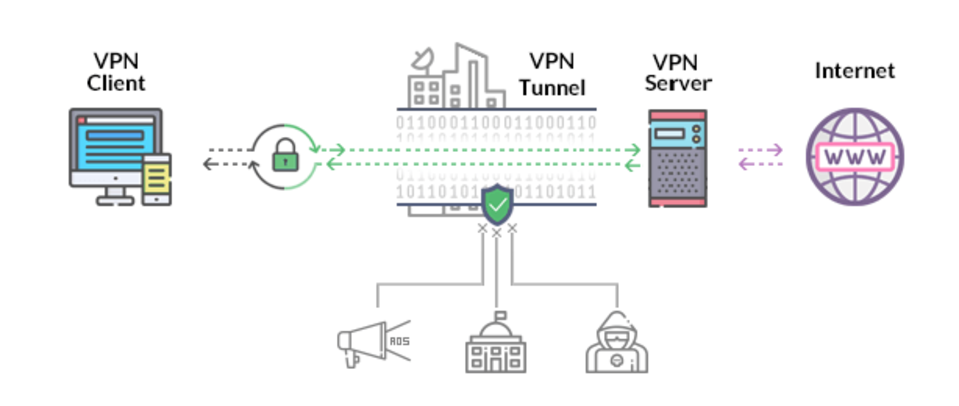
\includegraphics[width=0.95\linewidth]{figures/vpn_fancy}
	\caption{Ukážka typického VPN spojenia}
	\label{vpnfancy}
\end{figure}

\section{Výhody a nevýhody VPN sietí}
Medzi výhody VPN sietí patrí najmä zvýšenie bezpečnosti pripojenia. Všetka sieťová komunikácia je zašifrovaná pomocou kryptografického algoritmu. V závislosti od kvality implementácie sú informácie prenášané po takejto sieti nečitatelné. Ďalším typickým znakom je poskytnutie anonymity. VPN dokáže zamaskovať našu IP adresu a zároveň aj geografickú lokáciu. Tým, že sa pripojíme na~zariadenie v inej sieti, tak získavame prístup k všetkým povoleným zdrojom tohto vzdialeného zariadenia. Týmto spôsobom dokážeme napríklad pristupovať k interným dátam.
VPN je šikovný nastroj na ochranu vo verejnej nezabezpečenej sieti, ktorá bez VPN zabezpečenia poskytuje útočníkom rôzne možnosti útoku alebo zneužitia pripojeného zariadenia.

Medzi hlavné nevýhody patrí spomalenie internetového spojenia. Tým že, sa dodatočne spracúvavajú sieťové dáta, tak nastáva nechcené spomalenie. Táto dlhšia odozva siete sa predlžuje priamo úmerne od vzdialenosti servera, na ktorý sa pripájame. Ďalšou nepísanou nevýhodou je cena. Väčšina VPN poskytovateľov poskytuje služby za pomerne dráhe poplatky. Pri voľbe poskytovateľa je taktiež nutné prečítať si podmienky pripojenia. Niektorý poskytovatelia uchovávajú dáta, ktoré naprieč spojením prechádzajú. Poslednou nevýhodou je pomerne zložitá konfigurácia pri niektorých VPN protokoloch. Samozrejme, uvedený problém nastáva len pri prvotnej konfigurácií VPN siete.   

\section{Charakteristika a definovanie pojmov}
Obsahom tejto podkapitoly je zavedenie a následne stručná charakteristika pojmov, potrebných na pochopenie problematiky VPN sietí.
\subsection{Tunel a tunelovacie rozhrania}
\textbf{Tunel} v počítačových sieťach predstavuje virtuálne spojenie medzi jedným alebo viacerými zariadeniami. Jeho obsahom sa prenášajú zapuzdrené dáta (z~ang. \textit{encapsulated data}). Proces pridávania dát k pôvodným sa v tejto súvislosti zvykne taktiež označovať ako \textbf{tunelovanie}. V počítačových sieťach je týmto spôsobom možné zmeniť, resp. zameniť použitý protokol za iný. Príkladom by mohlo byť tunelovanie z IPv4 do IPv6. V uvedenom prípade sa z pôvodného paketu použijú dáta a k ním sa pridajú údaje potrebné na smerovanie v IPv6 sieti. Výhodou je, že týmto spôsobom vieme sprostredkovať kompatibilitu naprieč viacerými sieťami s~rôznymi protokolmi. Obdobne vieme do procesu tunelovania začleniť aj bezpečnostné prvky v podobe šifrovania a autentizácie pôvodných dát. V~súvislosti s~tunelmi sa používateľ môže stretnúť s pojmami tunelovací protokol a tunelovacie rozhranie. 

\textbf{Tunelovací protokol} predstavuje súbor činností, ktoré sá v procese tunelovania vykonávajú. V súčasnosti existuje veľa protokolov, ktoré sú štandardne špecifikované a bežne používané v sieťovej komunikácií. Najčastejšie sa používateľ stretne s tunelovaním pri VPN sieťach. Niektoré VPN v sebe nesú názov použitého tunelovacieho protokolu. Za spomenutie stojí protokol \textit{Generic Routing Encapsulation} (ďalej \acrshort{gre}). \acrshort{gre} je tunelovací protokol vyvinutý spoločnosťou Cisco v roku 1994. Ponúka širokú paletu možností tunelovania viacerých sieťových protokolov vo virtuálnych spojeniach medzi zariadeniami, tzv. z ang. \textit{point-to-(multi)point}. Niektoré variácie sa používajú aj pri vytváraní VPN. Viac informácií o \acrshort{gre} je dostupných na \cite{gre} a \cite{rfc1701}. 

\textbf{Tunelovacie rozhranie}, resp. adaptér je virtuálne zariadenie, ktoré je možné vytvárať v jadre daného operačného systému. Jedná sa o kompletne softvérové riešenie. Dôležité je, že nie každý \acrshort{os} má natívnu podporu pre vytváranie virtuálnych tunelovacích rozhraní. Je preto potrebné používať ovláďače tretích strán, ktoré danú funkcionalitu implementujú. Od roku 2000 podporujú tieto rozhrania Solaris, Linux a BSD operačné systémy. Poznáme dva typy virtuálnych softvérových tunelovacích rozhraní. Konkrétne \acrshort{tap} a \acrshort{tun} rozhranie. Nedajú sa použiť spolu, pretože pracujú na rôznych vrstvách. TUN emuluje správanie zariadenia na sieťovej vrstve (L3). Pracuje s paketmi a tie sa používajú pri smerovaní. Na druhej strane TAP rozhranie pracuje o úroveň nižšie s ethernetovými rámcami (L2). Používa sa na premostenie sieťovej komunikácie. TUN/TAP rozhrania je možné použiť na odosielanie a príjmanie dát. Dáta odoslané OS do TUN/TAP je možné modifikovať programom, ktorý rozhrania vytvoril. Na druhej strane používateľ môže v programe taktiež odoslať dáta do rozhraní. V tomto prípade TUN/TAP vloží dáta do sieťového zásobníka OS. Tým emuluje ich príjem z externého zdroja. 

Technológia TUN/TAP je pomerne známa a zaužívaná. Svoje uplatnenie zohráva pri softvérovej implementácií VPN. Okrem toho sa bežne používa aj v~sfére VM. Napríklad aj vo voľne dostupný nástroji na virtualizáciu -- VirtualBox. Pri vytvorení a následnom používaní obrazu VM, dochádza k vytváraniu tunelovacích rozhraní. Prostredníctvom zvolenej konfigurácie stroja sa rozhrania nakonfigurujú. Týmto spôsobom sa pre používateľa sprístupní možnosť komunikácie virtuálneho stroja s inými zariadeniami. 
Viac informácií o problematike je možné nájsť v \cite{tunel}, \cite{tuntap} a \cite{tun}, odkiaľ bol obsah tejto kapitoly čerpaný.     

\subsection{Charakteristika referenčných modelov}\label{crm}
Pred podkapitolou \ref{rm} je potrebné pred samotnou klasifikáciou vysvetliť pojmy Referenčný model prepojenia otvorených systémov (z ang. \textit{Open Systems Interconnection reference model}, ďalej \acrshort{osi}) a Model opisujúci balíky internetových protokolov (z ang. \textit{Transmission Control Protocol/Internet Protocol reference model}, ďalej \acrshort{tcpip}).

Úlohou uvedených referenčných modelov je vizualizácia postupu spracovania dát od používateľa až k ich odoslaniu zo zariadenia (z ang. \textit{end-to-end data communication}). Pojem spracovanie dát znamená opísanie toho, ako dochádza v~jednotlivých abstraktných vrstvách k pretransformovaniu používateľských dát na súbor jednotiek a núl, ktoré sú následne odoslané do iného zariadenia. 

\acrshort{osi} Model vznikol v skorších fázach evolúcie počítačových sietí. Vychádza skôr z teoretického než praktického prístupu. Pozostáva zo 7 abstraktných vrstiev (z ang. \textit{Layer}, ďalej \acrshort{l}):

\begin{enumerate}
	\item{\textbf{fyzická vrstva}} -- z ang. \textit{Physical Layer} (ďalej L1),
	\item{\textbf{spojová vrstva}} -- z ang. \textit{Data Link Layer} (ďalej L2), 
	\item{\textbf{sieťová vrstva}} -- z ang. \textit{Network Layer} (ďalej L3), 
	\item{\textbf{transportná vrstva}} -- z ang. \textit{Transport Layer} (ďalej L4), 
	\item{\textbf{relačná vrstva}} -- z ang. \textit{Session Layer} (ďalej L5), 
	\item{\textbf{prezenčná vrstva}} -- z ang. \textit{Presentation Layer} (ďalej L6), 
	\item{\textbf{aplikačná vrstva}} -- z ang. \textit{Application Layer} (ďalej L7). 
\end{enumerate}
V schéme, na~obrázku \ref{p2}, sa nachádzajú jednotlivé vrstvy spoločne so zariadeniami, ktoré pracujú s jednotlivými dátami. Zároveň je v obrázku znázornený proces rozbalenia (z ang. \textit{deencapsulation}). Schéma bola prevzatá z \cite{biks}.

\begin{figure}[h!]
	\centering
	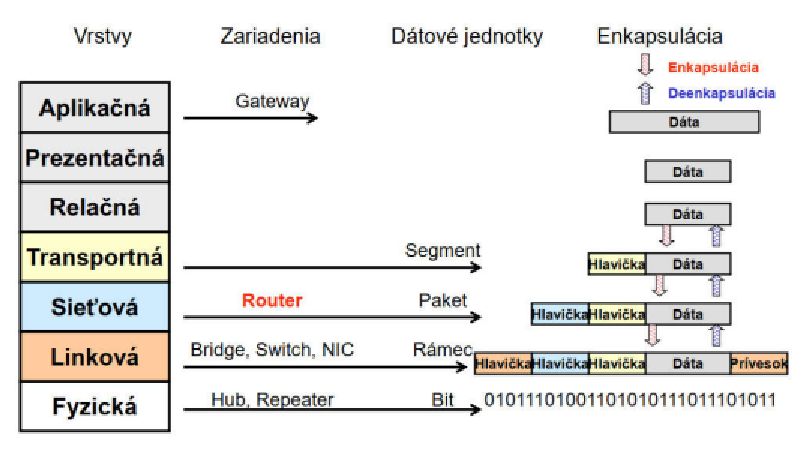
\includegraphics[width=0.9\linewidth]{figures/prenos2z2}
	\caption{Schéma postupného spracovania dát jednotlivými vrstvami OSI modelu \cite{biks}}
	\label{p2}
\end{figure}

Čím je väčšie číslo vrstvy tým bližšie sa dáta nachádzajú pri používateľovi. Vďaka uvedeným vlastnostiam je tento model vhodnejší pri začiatku štúdia spracovania sieťových dát v počítači. Z rovnakého dôvodu sa taktiež viac stretávame s jeho použitím pri opise funkcionality riešenia ako s novším \acrshort{tcpip} modelom.  Viac informácií o problematike nájde čitateľ v \cite{osi}.

Na druhej strane \acrshort{tcpip} model vznikol z praktického prístupu. Hlavný rozdiel je v počte abstraktných vrstiev, ktorý je v prípade \acrshort{tcpip} zmenšený na 4 vrstvy \cite{tcp}. 
TCP/IP model je zobrazený pomocou schémy na~obrázku \ref{tcpipprot}. V uvedenej schéme sú znázornené niektoré z protokolov, ktoré sa na jednotlivých vrstvách používajú.

\begin{figure}[!ht]
	\centering
	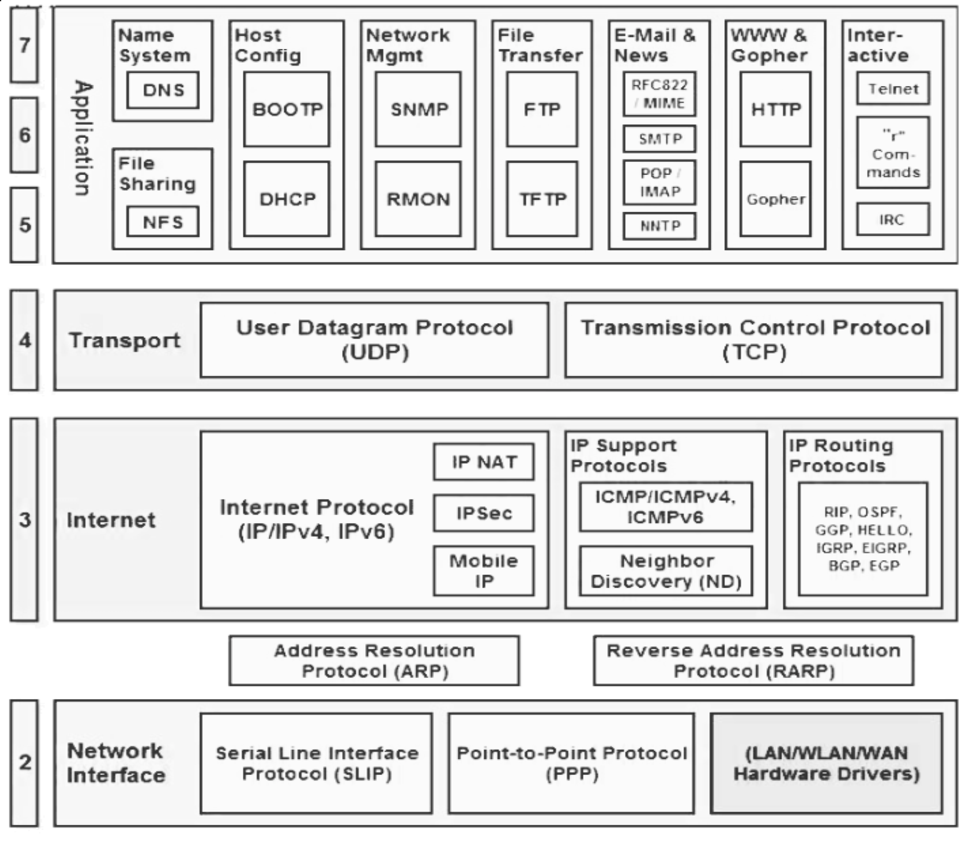
\includegraphics[width=0.9\textwidth]{figures/tcpiprot}
	\caption{Schéma TCP/IP modelu s niektorými protokolmi \cite{tcpguide}}
	\label{tcpipprot}
\end{figure}

\textbf{Aplikačná vrstva (L5-L7)} zahŕňa protokoly používané väčšinou aplikácií na~poskytovanie užívateľských služieb alebo výmenu aplikačných dát cez sieťové pripojenia, ktoré je vytvorené protokolmi na nižšej úrovni.  Spája vrstvy L5 až L7 OSI modelu. Príklady známych protokolov aplikačnej vrstvy sú \acrfull{http}, \acrfull{ftp}, \acrfull{smtp} a iné. Údaje, resp. dáta sú pri spracovaní kódované podľa L4 protokolov. Sú zapuzdrené do protokolových jednotiek transportnej vrstvy, tzv. \textbf{segmentov}.  

\textbf{Transportná vrstva (L4)} vytvára základné dátové kanály, ktoré aplikácie používajú na výmenu dát. Vrstva vytvára konektivitu medzi hostiteľmi, ktorá je nezávislá od siete, štruktúry užívateľských dát a smerovacích informácií. Konektivita na transportnej vrstve môže byť kategorizovaná ako orientovaná na spojenie, implementovaná v protokole \acrshort{tcp}, alebo \acrshort{udp} bez orientácie na spojenie. Uvedené protokoly sú stručne charakterizované nižšie, v tejto podkapitole. 

Protokoly v tejto vrstve zabezpečujú:
\begin{itemize}
	\item{riadenie chýb} -- z ang. \textit{error control} \cite{ec},
	\item{segmentáciu dát} -- z ang. \textit{segmentation} \cite{sd},
	\item{riadenie toku dát} -- z ang. \textit{flow control} \cite{fc},
	\item{riadenie preťaženia} -- z ang. \textit{congestion control} \cite{cc},
	\item{adresovanie aplikácií pomocou portov} -- z ang. \textit{application addressing} \cite{aa}.
\end{itemize}
Výstupom transportnej vrstvy sú segmenty, ktoré sú spracované v ďalšej vrstve referenčného modelu. 

\textbf{Internetová, resp. Sieťová vrstva (L3)} je zodpovedná za odosielanie paketov cez jednu alebo viac sietí. S touto funkcionalitou internetová vrstva umožňuje sieťovanie, prepojenie rôznych IP sietí a v podstate vytvára internet. Z L4 segmentov tvorí pakety, tak že pridá informácie potrebné na ďalšie smerovanie. 

\textbf{Linková vrstva (L1-L2)} sa používa na presun paketov medzi rozhraniami internetovej vrstvy dvoch rôznych hostiteľov na rovnakom linke. Procesy vysielania a prijímania paketov na linke je možné konfigurovať. Zariadenia nazývané prepínače (z~ang. \textit{switch}), vykonávajú rámcovania (z~ang. \textit{frame}). Pripravujú pakety z~vrstvy L3 na prenos pridaním ďalších informácií. Týmto úkonom vzniknú rámce. Tie sa prenášajú do~fyzickej vrstvy a cez prenosové médium až k hostiteľovi. Fyzická vrstva predstavuje prvok, cez ktoré sú dáta prenášane. Typickým príkladom je optický alebo ethernetový kábel. 

Vyššie uvedené procesy prípravy a spracovania dát sú znázornené pomocou schémy na~obrázku \ref{p1}. V tejto schéme je znázornený proces vytváranie sieťových dát, ich následne smerovanie naprieč sieťou a spracovanie v cieľovom zariadení. V bežnej prevádzke sa jedná o obojsmernú komunikáciu. Z uvedeného dôvodu sú šipky obojstranné. 

\begin{figure}[!h]
	\centering
	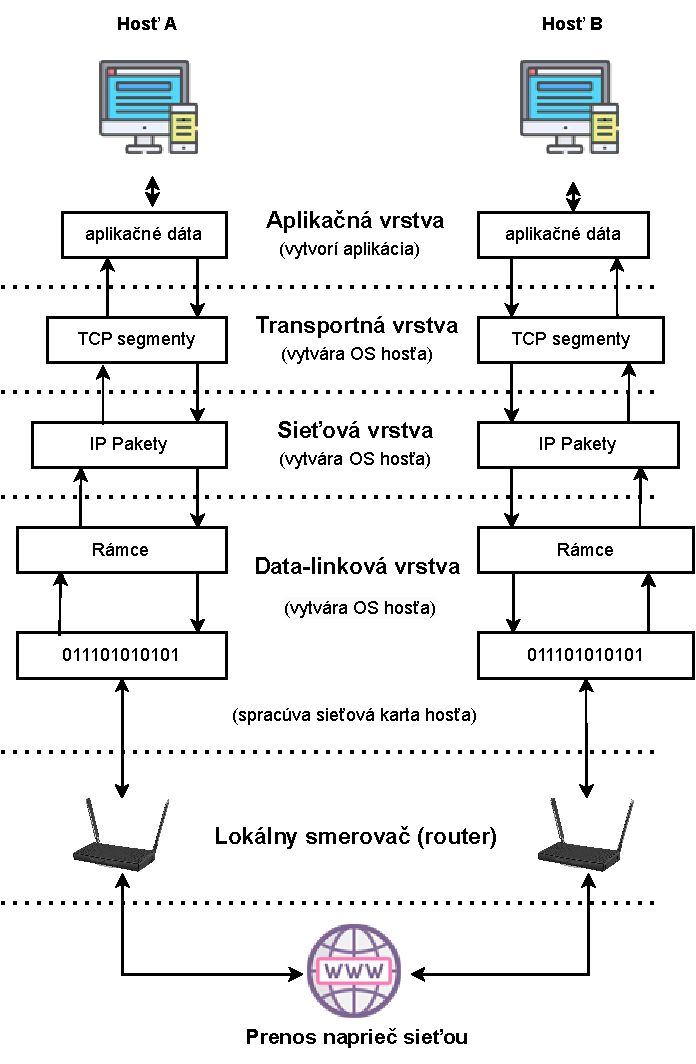
\includegraphics[width=0.8\linewidth]{figures/prenos1z2}
	\caption{Proces formovania a spracovania sieťových dát naprieč dvoma zariadeniami}
	\label{p1}
\end{figure}

\newpage
\textbf{Protokol riadenia prenosu} (z ang. \textit{Transmission Control Protocol}, ďalej \acrshort{tcp}) je komunikačný protokol orientovaný na nadviazanie a udržanie sieťového spojenia medzi zariadeniami. Môže byť použitý pri úlohe príjímateľa aj odosielateľa (z~ang. \textit{full-duplex}). Úlohou je spoľahlivý prenos dát medzi komunikantmi. Odoslanie a príjem dát je v rovnakom poradí. Protokol zároveň obsahuje mechanizmy na kontrolu výskytu chýb. Svoj názov má podľa dvoch najdôležitejších protokolov:
\begin{itemize}
	\item{Protokol riadenia prenosu} -- z ang. \textit{\acrlong{tcp}},
	\item{Internet protokol} -- z ang. \textit{\acrlong{ip}}. 
\end{itemize}

Na začiatku 21. storočia je 95\% paketov používaných na internete typu TCP. Bežné aplikácie používajúce TCP sú webové (HTTP/HTTPS protokoly), slúžiace na e-mailovú komunikáciu (SMTP/POP3/IMAP) a prenos súborov (z ang. \textit{File Transfer Protocol -- \acrshort{ftp}}). Minimálna dĺžka hlavičky TCP je 20 bajtov a maximálna dĺžka 60 bajtov. Po pridaní údajov TCP hlavičky k prenášaným dátam, vzniká tzv. \textit{segment}.

V súčasnosti je možne TCP protokol implementovať softvérovo aj hardvérovo. Pri prvom z uvedených je problémom závislosť na OS a následne aj vysoká vyťaženosť procesora pri príprave a spracovaní dát. Pri hardvérovom riešení je výhodou optimalizácia a implementácia bez potreby dodatočnej úpravy OS. Hardvérové implementácie sa realizujú pomocou koprocesorov.

Podrobnejšie informácie o TCP protokole je možné nájsť v \cite{tcp2}. V uvedenej publikácií sa nachádza opis TCP hlavičky, metódy nadviazania a ukončenia spojenia. Obdobne je spomenuté ako dochádza k prenosu dát pomocou sekvenčných čísel. V uvedenej publikácií a v \cite{tcpguide} môže čitateľ nájsť ďalšie informácie o protokole TCP.

\textbf{Používateľský datagramový protokol} (z ang. \textit{User Datagram Protocol}, ďalej \acrshort{udp}) je jedným zo základných komunikačných \acrshort{ip} protokolov. Používa sa na~odosielanie správ iným hostiteľom v~sieti. Správy sú prenášané ako datagramy v~paketoch. \acrshort{udp} nevyžaduje predchádzajúcu komunikáciu na~nastavenie komunikačných kanálov alebo dátových ciest. Používa jednoduchý komunikačný model bez spojenia s minimom protokolových mechanizmov. Poskytuje kontrolné súčty pre integritu údajov a čísla portov na adresovanie rôznych funkcií v zdroji a cieli datagramu. 

Narozdiel od \acrshort{tcp}) neposkytuje žiadnu záruka doručenia správy alebo duplicitnej ochrany. 
\acrshort{udp}) je vhodný na účely, kde kontrola a oprava chýb buď nie sú potrebné, alebo sa vykonávajú v aplikácii. Aplikácie citlivé na čas často používajú UDP, pretože zahadzovanie paketov je vhodnejšie ako čakanie na pakety oneskorené v dôsledku opätovného prenosu. Príklad použitia môžu byť streamovacie služby. 
Podrobnejšie informácie o \acrshort{udp} sú dostupné v \cite{udp}.

\section{Klasifikácia VPN sietí}
V súčasnosti má čitateľ k dispozícií veľa rôznych internetových zdrojov o problematike VPN. Uvedené sú rôzne možnosti klasifikácie VPN siete. V rámci tejto práce klasifikujeme VPN siete podľa logickej topológie a~vrstiev, na ktorých sú postupy aplikované. Obsahom tejto podkapitoly je rozdelenie a opis jednotlivých typov VPN sietí. Klasifikáciu zavedenú v tejto práci je možné vidieť na obrázku \ref{vpnklas}. V závere kapitoly sa nachádza sumárne zaradenie opísaných VPN protokolov do~uvedenej klasifikácie.

\begin{figure}[!ht]
	\centering
	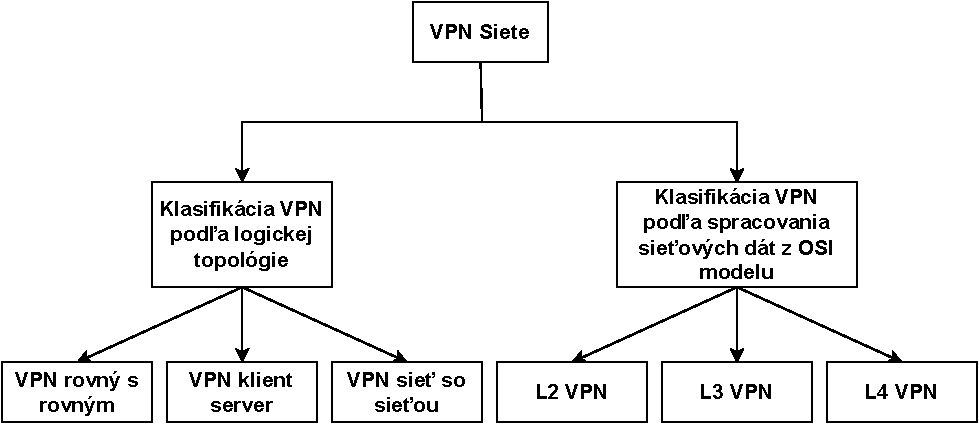
\includegraphics[width=\textwidth]{figures/vpnklas}
	\caption{Klasifikácia VPN sietí}
	\label{vpnklas}
\end{figure}
  
\subsection{Rozdelenie VPN sietí podľa logickej topológie}
 Podľa topológie, v ktorej VPN spojenie prebieha rozdeľujeme VPN do 3 kategórií: 
\begin{itemize}
	\item \textbf{VPN rovný s rovným} -- \textit{z ang. Peer to Peer VPN},
	\item \textbf{VPN klient a server} -- \textit{z ang. Client to Server VPN}, 
	\item \textbf{VPN sieť so sieťou} -- \textit{z ang. Site to Site VPN}.
\end{itemize}

\subsubsection{Topológia VPN siete typu rovný s rovným}
Uvedený spôsob vytvára zabezpečený tunel medzi dvoma rovnocennými \\uzlami, resp. zariadeniami (z ang. \textit{peers}), ktorí spoločne komunikujú cez verejnú sieť. Medzi zariadeniami je vytvorený tunel. Každý koniec má priradenú svoju IP adresu. Z uvedeného modelu vyplýva aj následné obmedzenie. VPN tunel vznikne iba medzi dvoma komunikujúcimi zariadeniami. Z toho dôvodu nie je toto použitie časté. Na obrázku \ref{p2p} je znázornený uvedený typ VPN spojenia. 
\begin{figure}[!ht]
	\centering
	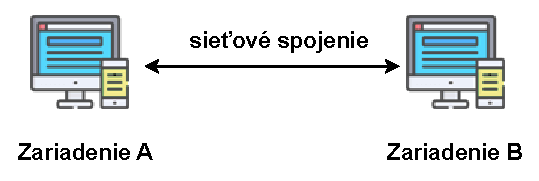
\includegraphics[width=.7\textwidth]{figures/p2p}
	\caption{Ukážka spojenia zariadení typu rovný s rovným}
	\label{p2p}
\end{figure}
 
\subsubsection{Topológia VPN siete typu klient a server}
Tento typ spojenia pozostáva z pripojenia medzi dvoma alebo viacerými nerovnocennými zariadeniami. Najjednoduchší model musí pozostávať z jedného VPN servera a VPN klienta. Princíp spočíva vo vytvorení zabezpečeného tunela, ktorý je použitý na prenos dát medzi uvedenými zariadeniami. Zároveň je VPN server schopný vytvoriť $N$ takýchto spojení. $N$ reprezentuje počet VPN klientov, s ktorými dokáže server nadviazať spojenie. Tento parameter je závislý najmä od~hardvérových prostriedkov daného servera.

Úloha klienta spočíva v presmerovaní všetkej svojej sieťovej komunikácie cez zabezpečený tunel, ktorý vznikol medzi ním a serverom. Tento úkon je najčastejšie realizovaný presmerovaním komunikácie cez sieťovú bránu (z ang. \textit{GateWay}, ďalej \acrshort{gw}). V danom \acrshort{os}, na ktorom VPN klient beží, je teda potrebné zmeniť IP adresu \acrshort{gw} na adresu VPN servera. Vďaka tomu nastane presmerovanie komunikácie. Tento úkon je väčšinou realizovaný programovo pomocou aplikácií. Typicky sa nadviaže spojenie medzi klientom a serverom. Následne sa upravia sieťové nastavenia systému. Spomenuté úkony sú vysoko závislé od \acrshort{os} a daného programovacieho jazyka, prostredníctvom ktorého sú úpravy realizované. 
Úloha servera na druhej strane spočíva vo vytvorení možnosti pripojenia pre jedného alebo viacerých klientov. Následne server zastupuje klientovu prítomnosť v danej sieti, spracúva požiadavky klienta a komunikuje s ostatnými zariadeniami. Komunikácia ďalej však už nie je zabezpečená pomocou šifrovania alebo tunelu. Na obrázku \ref{c2s} sa nachádza schéma pripojenie VPN klienta a servera.   

\begin{figure}[!h]
	\centering
	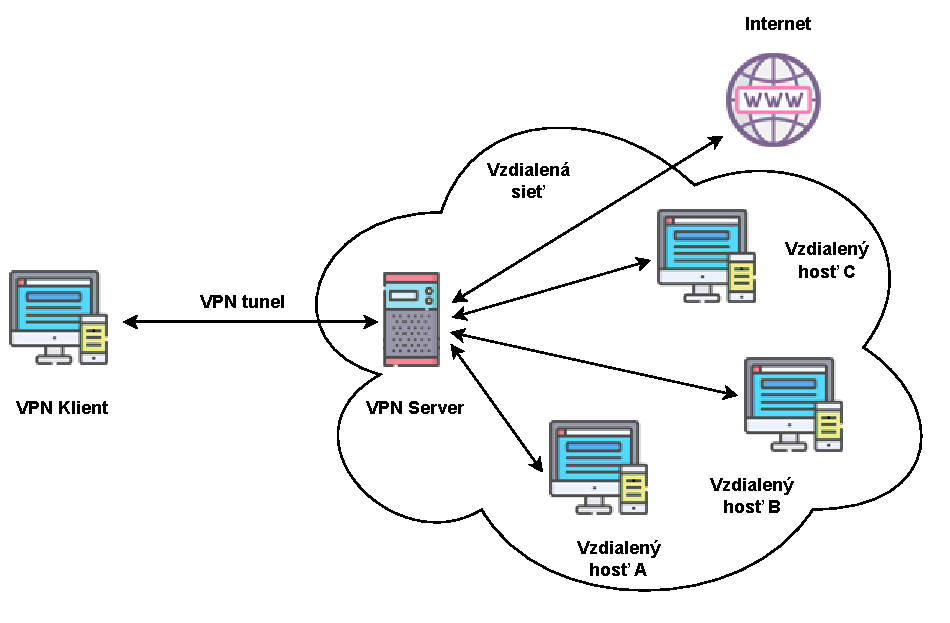
\includegraphics[width=\textwidth]{figures/c2s}
	\caption{Ukážka pripojenia VPN klienta na VPN server}
	\label{c2s}
\end{figure}
V súčasnosti je tento spôsob považovaný za najviac používaný. VPN server slúži ako vstupná brána do internej siete. Vďaka tomu je možné sprístupniť zdroje pre používateľov z rôznych oblastí sveta. Používateľ sa taktiež môže stretnúť s pomenovaním Model \textbf{uzol k sieti}, resp. z ang \textit{point-to-site}. Obdobne sa používa anglický výraz \textit{Remote access VPN}. Pojmy sú ekvivalentné a predstavujú rovnakú myšlienku zapojenia VPN.  
\subsubsection{Topológia VPN siete typu sieť so sieťou}
VPN model Sieť so Sieťou vytvára zabezpečený tunel medzi dvoma rôznymi sieťami naprieč verejnou sieťou. Model pozostáva z 2 zariadení -- VPN servera a VPN koncentrátora (z ang. \textit{VPN Concentrator}).

VPN koncentrátor je typ sieťového zariadenia, ktoré poskytuje zabezpečené VPN spojenie a doručenie dát. Zvyčajne je to špecializovaný smerovač (z ang. \textit{router}). Dokáže vytvárať veľké množstvo VPN tunelov. Používa sa na nadviazanie spojenia VPN typu sieť so sieťou. Funkcionalita koncentrátora pozostáva z: 
\begin{itemize}
	\item{nadviazania spojenia a konfiguráciu VPN tunela} -- z ang. \textit{Establish and Configure tunnels},
	\item{autentizáciu používateľa} -- z ang. \textit{Authenticate users},
	\item{priradenie IP adries používateľov k tunelom} -- z ang. \textit{Assign tunnel/IP addresses to users},
	\item{šifrovanie a dešifrovanie dát} -- z ang. \textit{Encrypt and Decrypt data},
	\item{zabezpečiť integritu doručenia} -- z ang. \textit{Ensure end-to-end delivery of data}.
\end{itemize}

Model Sieť so sieťou je používaný najmä v korporátnom svete pri spojení vedľajšej pobočky s hlavnou, ktoré sa nachádzajú na rozdielnych geografických lokalitách. Pomocou schémy, na~obrázku \ref{sts}, je znázornený tento model. 

 \begin{figure}[!ht]
 	\centering
 	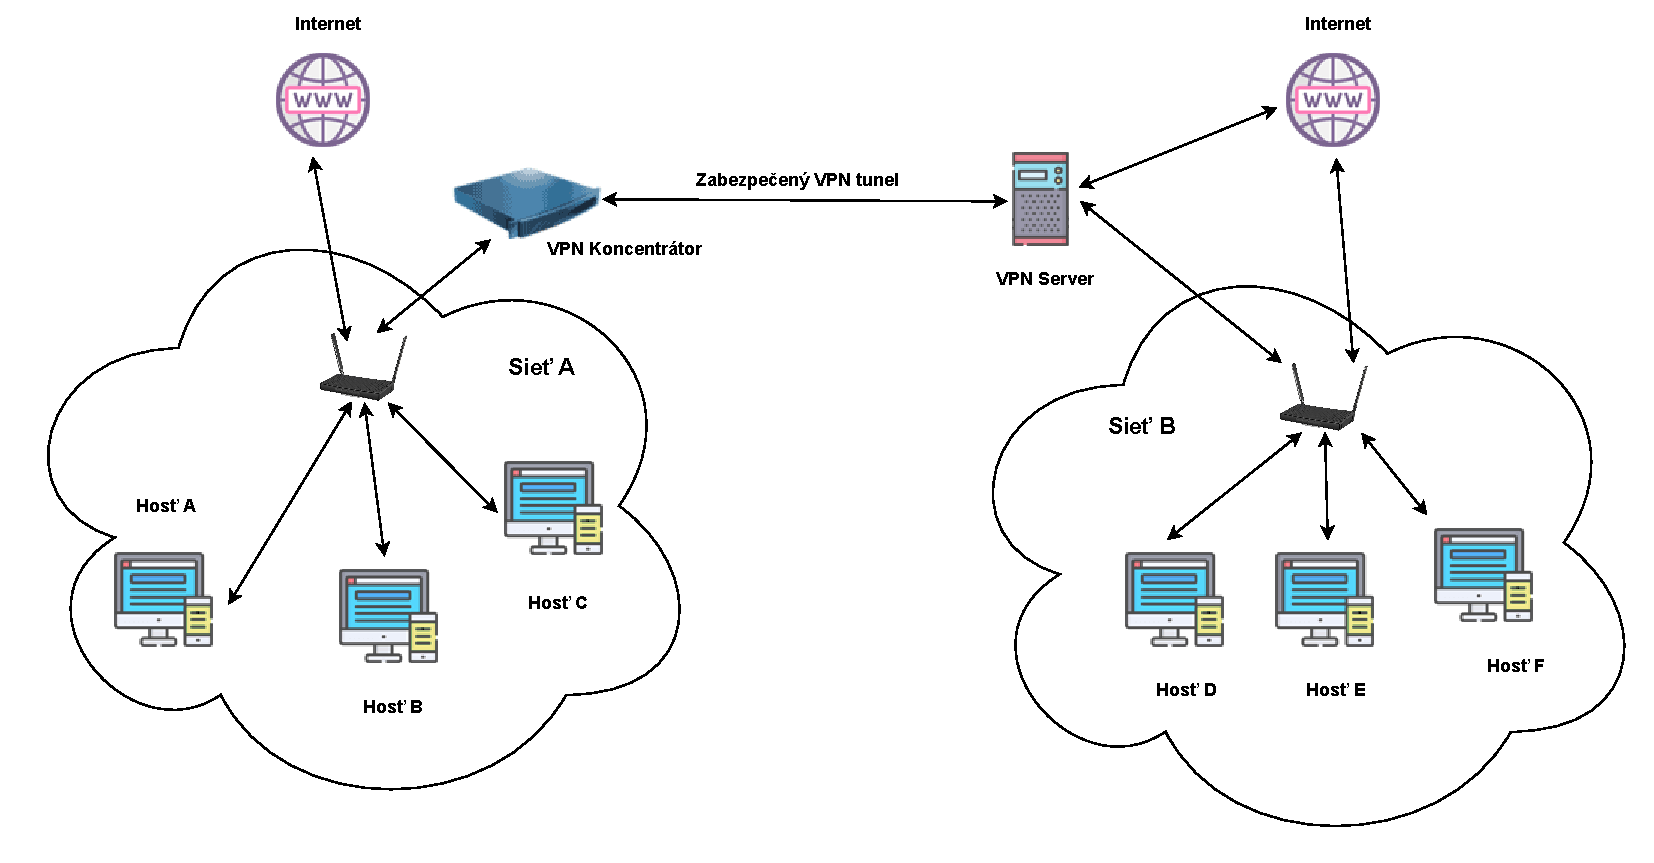
\includegraphics[width=1.1\textwidth]{figures/sts}
 	\caption{Ukážka spojenia VPN siete typu sieť so sieťou}
 	\label{sts}
 \end{figure}  
Používateľ však málo kedy pozná o aký presne druh VPN sa jedná. Najčastejšie sa stretne s označením, z ang. \textit{Remote Access VPN}. Jedná sa o vyššie uvedené VPN spojenie typu klient-server.

Informácia z tejto podkapitoly boli čerpané z \cite{vpntech}.  
\subsection{Rozdelenie VPN sietí podľa vrstiev referenčného modelu}\label{rm}
VPN siete môžeme klasifikovať aj podľa vrstvy (ďalej \acrshort{l}) referenčného modelu. Rozdelenie vytvoríme na základe vrstvy pôvodných sieťových dát, ktoré VPN aplikácia spracúva. Stručná charakteristika referenčných modelov je obsahom podkapitoly \ref{crm}. Každá dobrá VPN by v svojej implementácií mala realizovať šifrovanie. Preto použijeme túto činnosť ako príklad bloku, pri ktorom dochádza k už spomenutému spracovaniu pôvodných dát. 

Klasifikácia VPN sietí podľa \acrshort{osi} modelu:
\begin{itemize}
	\item{\textbf{L2 VPN}} -- VPN na spojovej vrstve,
	\item{\textbf{L3 VPN}} -- VPN na sieťovej vrstve,
	\item{\textbf{L4 VPN}} -- VPN na transportnej vrstve.
\end{itemize}

Pri implementácií VPN komunikácie medzi zariadeniami je pre pochopenie dôležité určiť aké dáta vstupujú do VPN algoritmu. Pomocou tejto informácie a~klasifikácie vyššie následne dokážeme zaradiť do určitej kategórie. 

Princíp použitia spracovania dát za pomoci bloku na šifrovanie je znázornený pomocou schémy na~obrázku \ref{sifr}. V schéme sa nachádzajú prerušované čiary. Tie reprezentujú scenár aký typ dát môže VPN spracúvať.

\begin{figure}[!h]
	\centering
	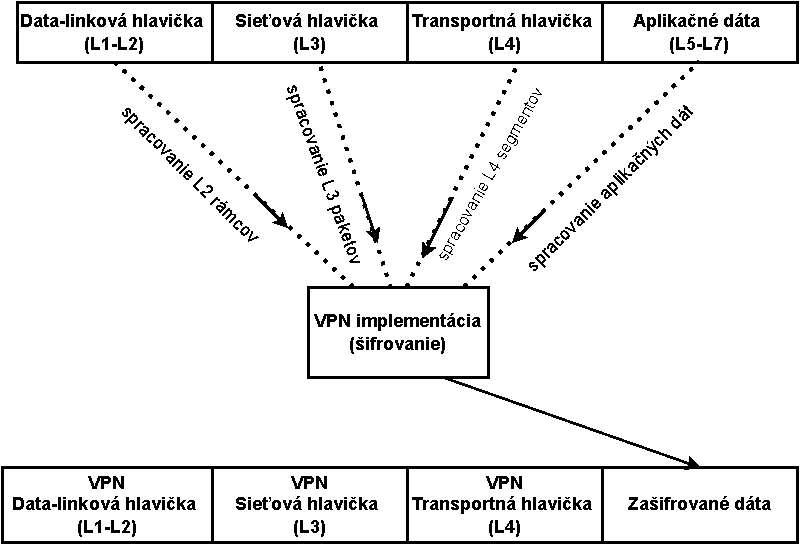
\includegraphics[width=1\textwidth]{figures/sifr}
	\caption{Ukážka formovania sieťových dát po spracovaní pôvodných dát}
	\label{sifr}
\end{figure}

Zo~schémy je viditeľné, že spracovaním nižšej vrstvy dochádza k zväčšeniu bloku dát, ktoré je potrebné spracovať. To môže negatívne ovplyvniť výslednú rýchlosť celého systému. Okrem uvedenej vlastnosti je ďalším problémom prenos vrámci rôznych sietí. Z uvedených dôvodov je preto najrozšírenejší spôsob VPN spracovania dát medzi vrstvami L3 až L4. 

Typicky sa s L2 a L3 VPN sieťami môže používateľ stretnúť v špecializovaných sieťových zariadeniach. Konkrétne na smerovačoch a prepínačoch. Prvé z~uvedených je využívané najmä pri smerovaní, respektíve určení cesty smerom z/do lokálnej siete až k cieľovej destinácií. Tento úkon je vykonaný za pomoci aplikácie smerovacích protokolov. Smerovač je možné použiť aj na smerovanie v~rámci lokálnej siete. V porovnaní s prepínačom však nedosahuje porovnateľný výkon. Na~druhej strane klasický prepínač je možné použiť len vrámci lokálnej siete. V~súčasnosti sa používajú aj tzv. L3 prepínače. V porovnaní so smerovačmi je ich prednosťou vyššia rýchlosť spracovania prichádzajúcich paketov pri väčšom počte pripojených zariadení. Všetky uvedené typy sa však dajú realizovať aj na~konečnom zariadení v podobe softvérovej implementácie.        

\section{Protokoly vo VPN sieťach} 
V predchádzajúcej podkapitole sme klasifikovali VPN siete na základe zapojenia kryptografického bloku do OSI referenčného modelu. V tejto podkapitole pomocou uvedeného rozdelenia, zaradíme a charakterizujeme niekoľko protokolov, ktoré sa typicky používajú vo VPN sieťach. Aktuálne neexistuje svetový štandard na vytváranie VPN spojení. Dôsledkom toho existuje veľké množstvo rôznych protokolov. V rámci tejto podkapaitoly si predstavíme niektoré z nich. 

\subsection{\acrfull{pptp}}
PPTP umožnuje vytvoriť zabezpečené VPN spojenie k inej internetovej sieti. \acrshort{pptp} používa \acrshort{tcpip}. \acrshort{tcpip} sieťový protokol zabezpečuje bezpečný prenos dát z klienta do privátneho servera vo VPN sieti. Jedná sa o starší Microsoft L2 protokol, ktorý bol definovaný v roku 1996. Je rozšírením L2 \acrshort{p2p} protokolu. \acrshort{pptp} zapuzdruje \acrshort{p2p} rámce do  IP paketov. Následne ich prenáša cez sieť. 

Zabezpečenie prenosu pomocou \acrshort{pptp} pozostáva typicky z 3 po sebe nasledujúcich procesov:
\begin{enumerate}
	\item{PPP pripojenie a komunikácia } -- z ang. \textit{PPP Connection and Communication},
	\item{riadenie spojenia pomocou PPTP protokolu} -- z ang. \textit{PPTP Control Connection},
	\item{prenos dát PPTP tunelom} -- z ang. \textit{PPTP Data Tunneling}.
\end{enumerate}
Prechod medzi procesmi je možný len ak došlo k úspešnému dokončeniu predchádzajúceho kroku. V prvom procese sa PPTP klient pripája k serveru s prístupom na internet (z ang. \textit{Network Access Server}, ďalej \acrshort{nas}). Používa sa pri tom PPP protokol, ktorý nadviaže spojenie a zašifruje pakety. V druhom kroku následne vznikne TCP pripojenie medzi NAT a PPTP serverom. Použité je číslo portu 1723. Uvedeným postupom nám vznikne medzi zariadeniami PPTP Tunel. Po úspešnom vytvorení konektivity dochádza k zapuzdrovaniu prichádzajúcich zašifrovaných PPP dát do PPTP protokolu a ich prenosu cez tunel. PPTP zapuzdruje dáta do tzv. IP datagramov, ktoré už obsahujú zašifrovaný PPP paket. Datagramy su vytvorené pomocou \acrshort{gre} protokolu, ktorý bol spomenutý na začiatku. Na~obrázku \ref{pptpdat} je znázornený PPTP rámec. 

\begin{figure}[!h]
	\centering
	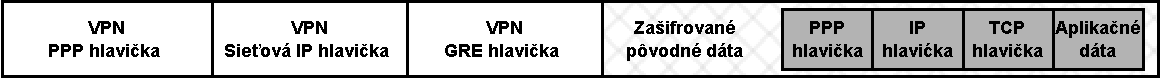
\includegraphics[width=\textwidth]{figures/pptpdat}
	\caption{Schéma zložených sieťových dát po PPTP spracovaní}
	\label{pptpdat}
\end{figure}

PPTP server po prijatí dáta rozbalí, dešifruje PPP paket a následne ho smeruje v rámci lokálnej siete.

Je dôležité poznamenať, že PPTP klient môže mať priamy prístup na internet. V uvedenom prípade sa nevytvára prvotné PPP spojenie až k internetovému poskytovateľovi.
Viac informácií o protokole PPTP sa nachádza v \cite{rfc2637} a \cite{pptp}, ktoré boli zdrojom pri tvorbe tejto podkapitoly.
\subsubsection{Bezpečnosť a použitie protokolu} 
Protokol vznikol v júni 1996. Implementácia poskytuje používateľovi:
\begin{itemize}
	\item{\textbf{Autentizáciu}} -- z ang. \textit{Authentication}, overenie totožnosti používateľa pomocou mena a hesla. Na výber boli autentizačné protokoly \textit{Challenge Handshake Authentication Protocol} (\acrshort{chap}) \cite{chap}, \textit{MicroSoft Challenge Handshake Authentication Protocol} (\acrshort{mschap}) \cite{mschap} a \textit{Password Authentication Protocol} (\acrshort{pap}) \cite{pap}.  
	\item{\textbf{Kontrolu prístupu}} -- z ang. \textit{Access Control}, po úspešnej autentizácií je následne prístup používateľa riadený na základe pravidiel a politiky prístupu daného OS. 
	\item{\textbf{Šifrovanie dát}} -- z ang. \textit{Data Encryption}, je vykonané pomocou vopred zdieľaného kľúča, ktorý sa získa odvodením z hašovanej hodnoty uloženého hesla používateľa. Haš je vstupom do prúdovej šifry RC4 \cite{rc4} a výstupom je  40-bitový kľúč relácie. 
	\item{\textbf{Filtrovanie PPTP paketov}} -- z ang. \textit{PPTP Packet Filtering}, možnosť zapnutia filtrovania paketov len autentizovaných PPTP klientov.
	\item{\textbf{Preddefinované Firewall pravidla pre PPTP}} -- z ang. \textit{PPTP with Firewalls and Routers}, PPTP má štandardne definované číslo TCP portu 1723 a ID 47 v IP protokole. Vďaka tomu je možné jednoducho presmerovať tok dát.
\end{itemize} 

Protokol je aktuálne štandardne zahrnutý v každej distribúcií \acrshort{os} Windows aj Linux. Pri vytváraní VPN siete teda používateľ môže zvoliť uvedený protokol na~zabezpečený prenos dát v lokálnej, ale aj naprieč verejnou sieťou. Výhodou protokolu je vysoká kompatibilita naprieč rôznymi platformami. Nevýhodou je veľké množstvo zraniteľných miest, možností zneužitia a použitie starších kryptografických algoritmov. Aktuálne existujú protokoly poskytujúce lepšiu bezpečnosť ako uvedená implementácia. Z uvedených dôvodov sa tento protokol neodporúča používať.


\subsection{\acrfull{l2tp}}
Ďalším z VPN tunelovacích protokolov je \acrshort{l2tp}. Špecifikovaný bol v~roku 2000 v~dokumente \acrshort{rfc} (z~ang. \textit{Request For Comments}) 2661 \cite{rfc2661}. Inšpirovaný dvoma staršími protokolmi \acrshort{l2f} (z~ang. \textit{Cisco Layer 2 Forwarding Protocol}) \cite{rfc2341} a PPTP.   

L2TP sieť pozostáva primárne z 3 zariadení:
\begin{enumerate}
	\item{\textbf{PPP terminál}} -- ľubovoľné zariadenie na vykonanie PPP zapuzdrenia na dáta a pripojenie k \acrshort{lac} (z ang. \textit{L2TP Access Concentrator}). Môže to byť aj samotné zariadenie, ktoré sa pripája. 
	\item{\textbf{L2TP prístupového servera}} -- \acrshort{lns} (z ang. \textit{L2TP Network Server}), jeden z koncov tunela, ktorý rozbalí dáta a poskytuje prístup do lokálnej sieti. Na zariadení prebieha autentizácia používateľa, vytvorenie PPP relácie (z ang. \textit{session}) a L2TP tunela s \acrshort{lac}. Nasadzuje sa na hranici medzi privátnou a verejnou sieťou, zvyčajne ako sieťová brána na opustenie danej súkromnej siete (z ang. \textit{gateway}). Obdobne poskytuje funkcionalitu prekladu adries z privátnych do verejných a opačne. Uvedená funkcionalitá sa nazýva \acrfull{nat}. Viac o tomto protokole je dostupné na \cite{nat}.   
	\item{\textbf{L2TP koncentrátora}} -- \acrshort{lac}, zariadenie umiestnené medzi LNS a clientom. Služí na preposielanie paketov oboma smermi. V smere k LNS vytvára L2TP tunel. LAC server môže byť nasadený aj na PPP termináli a pracovať ako \acrshort{poe} (z ang. \textit{PPP Over Ethernet}) server.
\end{enumerate}
Na~obrázku \ref{l2tp} je znázornené schéma, ako sú spomenuté zariadenia zapojené v logickej topológií. V~obrázku je znázornený aj proces zapuzdrenia PPP paketov, prenosu dát naprieč tunelom a následného rozbalenia. Schéma bola mierne poupravená a prevzatá z \cite{l2tphuawei}. 
% TODO: \usepackage{graphicx} required
\begin{figure}[!h]
	\centering
	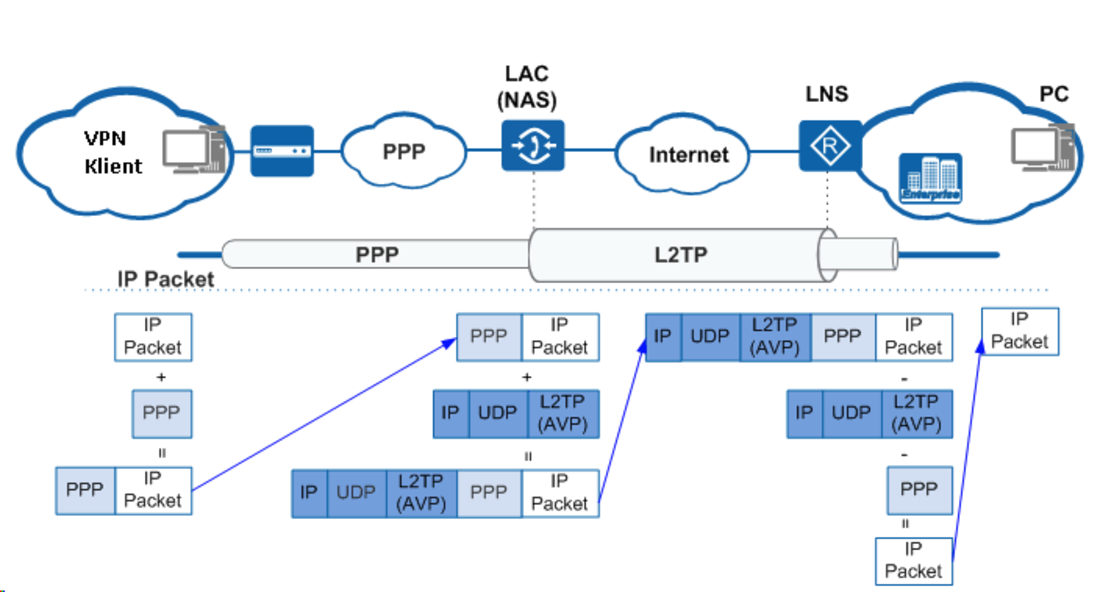
\includegraphics[width=1\textwidth]{figures/l2tp}
	\caption{Proces tunelovanie naprieč L2TP VPN protokolom \cite{l2tphuawei}}
	\label{l2tp}
\end{figure}

L2TP používa namiesto TCP protokolu UDP, ktorého výhodou je rýchlejší prenos bez kontroly prijatia na druhej strane spojenia.  
Pri vzniku tunela používa UDP port 1701. Iniciátor tohto procesu následne vyberá náhodne z nečinných portov a smeruje nim pakety s portom 1701. Prijímač po prijatí paketu taktiež náhodne určí nečinný port a preposiela ním pakety prijaté iniciátorom. Takto zvolené číslo portu sa používa až kým nie je komunikácia cez tunel ukončená. 

L2TP vytvára 2 druhy spojenia počas vytvárania konektivity medzi LAC a~LNS. 
\begin{itemize}
	\item{\textbf{tunelové spojenie}} -- z ang. \textit{tunnel connection}, napomáha k nastoleniu viacero tunelov medzi zariadeniami. Pozostáva z jedného alebo viacerých relačných spojení. Žiadosť o vytvorenie vytvára LAC server po prijatí PPP žiadosť od vzdialeného používateľa. LAC a LNS si vymenia informácie potrebné na vznik spojenia ako sú napríklad autentizačné informácie tunela a ID. Po úspešnom vyjednávaní (z ang. \textit{negotiation}) vznikne tunel, ktorý je identifikovateľný pomocou dohodnutého ID.  
	\item{\textbf{relačné spojenie}} -- z ang. \textit{session connection}, reprezentuje PPP spojenie naprieč tunelom. Môže vzniknúť až keď je tunel úspešne vytvorený.	
\end{itemize}     
Po vytvorení oboch spojení následne odchádza k prenosu zapuzdrených PPP paketov naprieč týmto tunelom.

L2TP ponúka kompatibilitu pre mnohé platformy a jednoduchú konfiguráciu. OS Windows, Linux a Mac majú tento protokol zabudovaný v sebe. Výhodou je použitie UDP, vďaka tomu je možné protokol používať aj v nestabilnom sieťovom prostredí.
Nevýhodou je zníženie prenosovej rýchlosti. L2TP používa taktiež vopred zdieľané kľúče a v prípade ak sa nezhodujú, tak dochádza k zastaveniu chodu. L2TP podporuje iba limitovaný počet portov. Samotná implementácia L2TP neposkytuje, respektíve nezabezpečuje žiadne šifrovanie alebo autentizáciu paketov. Na zabezpečenie sa používa v kombinácií s iným protokolom. Veľmi známa je implementácia L2TP/IPSec. 

V roku 2005 vznikla 3. verzia protokolu, ktorá priniesla zväčšenie dĺžky ID v~L2TP hlavičke, zo 16 na 32 bitov. Rozšírenie tunelového autentizačného mechanizmu a oddelenie L2TP dát súvisiacich s PPP protokolom. Viac o tomto upravenom protokole je možné nájsť na \cite{l2tpv3}.
  
Viac informácií o L2TP problematike je možné nájsť v \cite{l2tp}, \cite{rfc2661}, \cite{l2tphuawei}, odkiaľ boli informácie z tejto podkapitole čerpané. 

\subsection{Internet Protocol Security (\acrshort{ipsec})}
\acrshort{ipsec} je otvorený štandard. Vďaka tomu vďačí za veľkú popularitu a pravidelné aktualizácie kryptografických algoritmov. Protokol sa využíva na zabezpečenie bezpečnosti v sieti. IPSec môžeme klasifikovať ako L3 protokol, keďže pracuje s dátami zo sieťovej vrstvy. Má dva režimy:
\begin{itemize}
	\item{\textbf{transportný režim}} -- po prijatí paketu z vyššej vrstvy sú smerovacie dáta zachované a na základe nich sú dáta odosielané ďalej. K zvyšným dátam je pridaná hlavička použitého IPSec protokolu. Princíp pridania sieťových dát k pôvodným je znázornený na \ref{iptransport}.  
	\item{\textbf{tunelovací režim}} -- zapuzdruje paket. Pridáva novú IP hlavičku a hlavičku IPSec protokolu (ESP/AH) k pôvodnému nezapuzdrenému paketu. Uvedená skutočnosť je zobrazená na obrázku \ref{iptunel}.
\end{itemize}
% TODO: \usepackage{graphicx} required
\begin{figure} [!h]
	\centering
	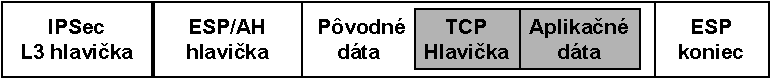
\includegraphics[width=\textwidth]{figures/iptransport}
	\caption{IPSec transportný režim}
	\label{iptransport}
\end{figure}
% TODO: \usepackage{graphicx} required
\begin{figure} [!h]
	\centering
	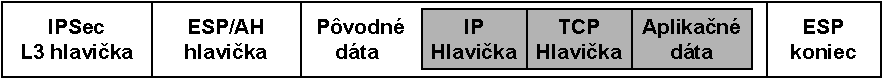
\includegraphics[width=\textwidth]{figures/iptunel}
	\caption{IPSec tunelovací režim}
	\label{iptunel}
\end{figure}


Za účelom poskytnutie zabezpečeného spojenia, protokol vykonáva autentizáciu, šifrovanie a vyjednávanie (z ang. \textit{negotiation}), resp. výmenu potrebných kľúčov. Jednotlivé činnosti sú realizované pomocou týchto IPSec protokolov:
\begin{itemize}
	\item{\textbf{Autentizačná hlavička}} -- z ang. \textit{Authentication Header}, pridáva k prepravovanému paketu dáta na zabezpečenie dátovej integrity a pôvodu. Chráni proti z ang. \textit{Replay attack} \cite{repa}. Dáta v tomto režime nie sú šifrované. AH hlavička je vygenerovaná v závislosti od toho v akom IPSec režime je protokol použítý.    
	\item{\textbf{Bezpečnostné zapuzdrenie nákladu}} -- z ang. \textit{Encapsulating Security Payloads}, narozdiel od AH, ESP aj šifruje dáta z vyššej vrstvy. Vďaka tomu dochádza k zabezpečeniu dôvernosti, datovej integrity a autentizácie pôvodu. Výsledná hlavička závisí od dát zo sieťovej vrstvy a konfigurácie IPSec.    
	\item{\textbf{\acrlong{isakmp}}} -- ďalej \acrshort{isakmp}, protokol na autentizáciu a výmenu kľúčov. Slúži taktiež na vytvorenie parametra \acrshort{sa}, ktorý sa používa v hlavičke \acrshort{ah}/\acrshort{esp}.
\end{itemize}

IPSec je možné nakonfigurovať, tak aby používal \acrshort{ah} a \acrshort{esp} selektívne alebo aj súčasne. V závislosti od konfigurácie následne dochádza k zapuzdrovaniu prichádzajúceho paketu. Používateľ má na výber viacero štandardných kryptografických algoritmov. Príkladmi sú \acrshort{aes} \cite{aes}, \acrshort{rsa} \cite{rsa}, Diffie-Hellman \cite{dh} a  eliptické krivky (\acrshort{ecdsa} \cite{ecdsa} aj \acrshort{ecdh} \cite{ecdh}).

\subsection{Secure Socket Tunneling Protocol (\acrshort{sstp})}
SSTP je bežný L2 VPN protokol, ktorý zapuzdruje PPP rámce cez \acrshort{https} protokol \cite{https}. Spolieha sa na \acrshort{ssl}, resp. \acrshort{tls}, ktoré sú opísané neskôr v práci. Vďaka tomu umožňuje ľahší prechod cez väčšinu firewallov a proxy brán. Teda blokovanie takto vytvoreného VPN spojenia je pre poskytovateľov internetu a správcov siete zložitejšie. 

SSTP bol vytvorený v roku 2007 spoločnosťou Microsoft. Primárne pre platformu Windows. Cieľom bolo poskytnúť bezpečnejšiu náhradu za PPTP a L2TP. V súčasnosti sa považuje za jeden zo štandartných protokolov. Je dostupný vo~viacerých operačných systémoch vrátane Linuxu a BSD. Protokol je pravidelne udržiavaný o~čom svedčí aj priebežná aktualizácia dokumentácie na Microsoft dokumentačných stránkach. Informácie k tejto podkapitole boli čerpané z \cite{mssstp}. V uvedenom zdroji je možné nájsť podrobnejšie informácie o protokole. 

Proces zapuzdrenia dát s využitím protokolov je znázornený pomocou obrázka \ref{sstpprotocolstack}. 
% TODO: \usepackage{graphicx} required
\begin{figure}[!h]
	\centering
	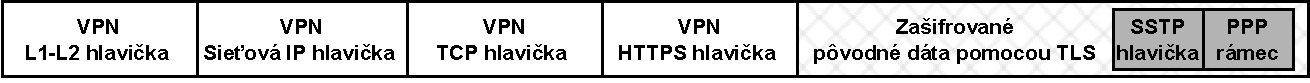
\includegraphics[width=1\textwidth]{figures/sstpprotocolstack}
	\caption{Proces zapuzdrenia pôvodných PPP rámcov naprieč SSTP protokolom}
	\label{sstpprotocolstack}
\end{figure}
Pri vytváraní SSTP segmentu dochádza k zapuzdreniu PPP rámcov pomocou HTTPS s využitím TCP protokolu s číslom portu 443. Po úspešnom nadviazaní TCP a overení SSL/TLS spojenia dochádza k spracovaniu SSTP hlavičky. Po úspešnom odstránení sa následne získa prístup k pôvodnému PPP rámcu.   

Podobne ako tomu bolo v prípade L2TP protokolu, opísaného vyššie, tak z hľadiska prenosu sa prenášajú naprieč tunelom dva druhy paketov. Vytvára a odosiela ich klient aj server. Majú špecifický formát a musia byť prenášané po bajtoch a v sieťovom poradí bajtov (z ang. \textit{network byte order}), z ľava do prava, teda od najvýznamnejšieho bitu po najmenej významný\footnote{sieťové spracovanie dát známe aj ako z ang. \textit{Big Endian}}. Prvé 4 parametre v oboch hlavičkách sú rovnaké: 
\begin{enumerate}
	\item{\textbf{Verzia}} -- z ang. \textit{Version}, má veľkosť 8-bitov, používa sa pri komunikácií a vyjednávaní SSTP verzie, ktorá sa má použiť. Prvé 4 bity signalizujú majoritnú verziu a zvyšné minoritnú verziu. 
	\item{\textbf{Reservované}} -- z ang. \textit{Reserved}, 7 bitov nastavených na 0, rezervované pre budúce použitie, pri spracovaní sa ignorujú.
	\item{\textbf{C}} -- 1 bit, indikátor pre dátový (0) a kontrolný SSTP paket (1). 
	\item{\textbf{Dĺžka paketu}} -- z ang. \textit{LengthPacket}, 16-bitový parameter, pozostáva z:
		\begin{itemize}
			\item{\textbf{R}} -- 4 bity, pripravené na budúce použitie, nastavené na 0 a ignorované,
			\item{\textbf{Dĺžka}} -- z ang. \textit{Length}, 12 bitov, špecifikuje bajtovú veľkosť celého SSTP paketu.
		\end{itemize}
\end{enumerate}
 
Rozdielnosť medzi hlavičkami vzniká v:
\begin{itemize}
	\item{\textbf{Dátové SSTP pakety}} -- z ang. \textit{SSTP Data Packets} \cite{datpak}, obsahujú 5. parameter 
		\begin{itemize}
			\item{\textbf{5. Dáta}} -- pole variabilnej dĺžky. Obsahuje zapuzdrený náklad z vyššej vrstvy.
		\end{itemize} 
	\item{\textbf{Kontrolné SSTP pakety}} -- z ang. \textit{SSTP Control Packets} \cite{conpak}, obsahuje 3 dodatočné parametre:
		\begin{itemize}
			\item{\textbf{5. Typ správy}} -- z ang. \textit{Message Type}, 16-bitové pole s SSTP správou o stave spojenia. Celkovo 9 možných správ \cite{conpak}. 
			\item{\textbf{6. Číselné atribúty}} -- z ang. \textit{Num Attributes}, 16-bitové pole, ktoré špecifikuje počet parametrov v správe.
			\item{\textbf{7. Atribúty}} -- z ang. \textit{Atributes}, zoznam parametrov s variabilnou veľkosťou.
		\end{itemize}	
\end{itemize}   
 
Protokol vo všeobecnosti nepodporuje spojenie typu sieť k sieti. Primárne je orientovaný na pripojenie klienta k sieti, za účelom získania vzdialeného prístupu. To isté platí pri autentizácií. Je možné autentizovať iba používateľa, iné možnosti nie sú podporované (zariadenie, smart card, počítať,...). V prípade nestabilného spojenia, je možný vysoký výskyt straty paketov. Dôvodom je použitie TCP protokolu. 

Bezpečnosť SSTP je sprostredkovaná za pomoci HTTPS protokolu, ktorý používa SSL/TLS. Aplikované kryptografické algoritmy závisia od verzie SSL/TLS, ktorá je použitá v implementácií. TLS bol predmetom opisu v úvode práce. SSTP sa považuje za veľmi bezpečný protokol. Na druhej strane použitie robustných šifrovacích a autentizačných algoritmov, dosť spomaľuje výsledné SSTP VPN pripojenie.

Viac informácií o protokole môže čitateľ nájsť v \cite{mssstp}, odkiaľ boli aj informácie pre túto podkapitolu čerpané.  

\subsection{Transport Layer Security -- TLS}
TCP ani UDP protokol sam o sebe nezabezpečí dáta, ku ktorým sa pridáva hlavička. Dôsledkom toho vznikli viaceré protokoly slúžiace na autentizované šifrovanie aplikačných dát. Najznámejší je protokol zabezpečenia prenosu -- \acrshort{tls}. 

Zabezpečenie dát bolo prvotne vykonávané pomocou protokolu \textit{Secure Sockets Layer} -- \acrshort{ssl}. Tento spôsob používa certifikáty na overenie pôvodcu dát. SSL malo od svojho vytvorenia dlhý vývoj, ktorý smeroval až k doteraz najpoužívanejšiemu TLS vo verzii 1.3. Ten vznikol v roku 2018. Inými slovami, TLS protokol je nástupca SSL pričom obsahuje rôzne úpravy a vylepšenia najmä z hľadiska rýchlosti. Zároveň sa v dnešnej dobe neodporúča používanie SSL protokolu. Dôsledkom optimalizácií je, že klienta komunikujúci so serverom cez HTTPS protokol s TLS 1.3 je rýchlejší ako v prípade použitia nešifrovaného HTTP variantu. 

Aktuálne je ešte podporovaná aj verzia TLS 1.2, ktorá vznikla v roku 2008. V čase tvorby práce ešte nebol ohlásený oficiálny dátum s ukončením jej podpory. Pri vývoji softvéru sa preto programátorom odporúča použiť najnovšiu verziu. 

TLS pracuje medzi aplikačnou a transportnou vrstvou. Spôsob spracovania dát je zobrazený pomocou obrázka \ref{ssl} s SSL operáciami, prevzatého z \cite{biks}. Postup v SSL a TLS ostáva zachovaný.
 
\begin{figure}[!ht]
	\centering
	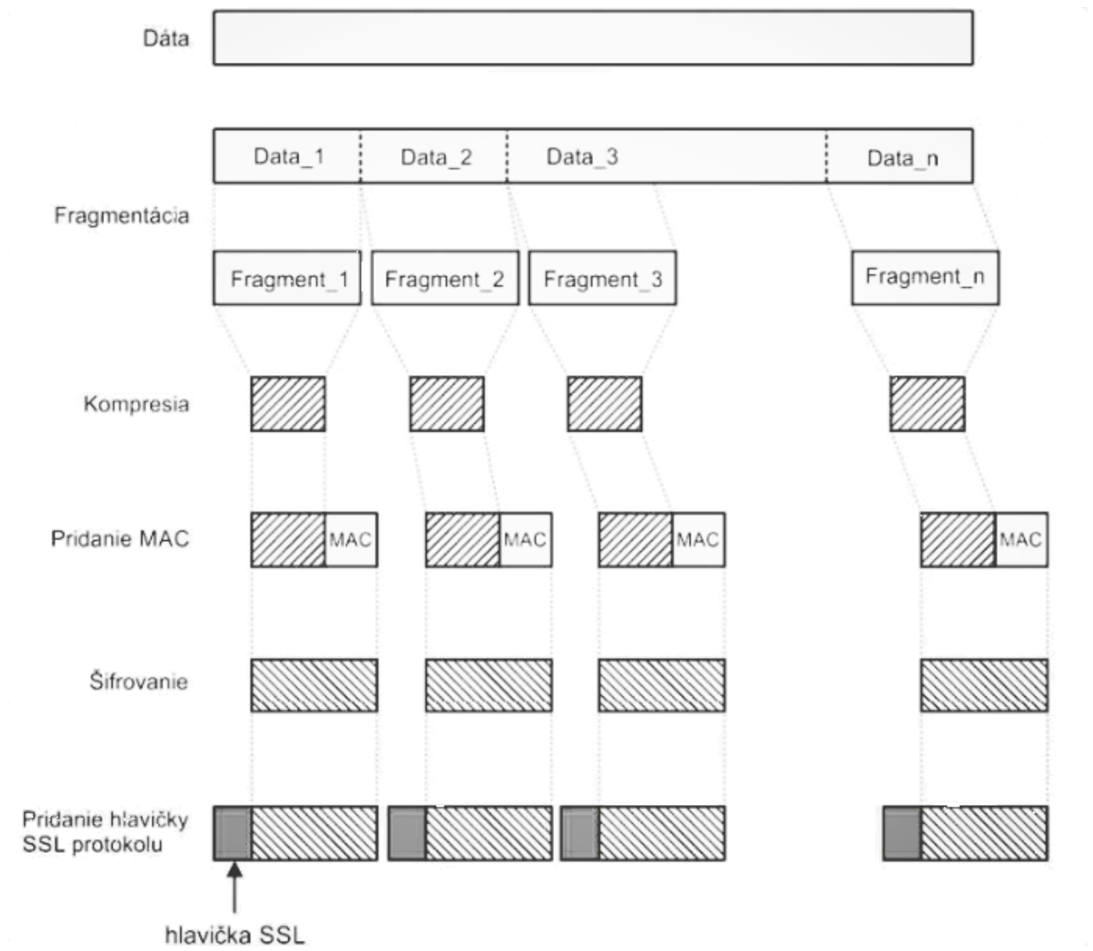
\includegraphics[width=0.8\linewidth]{figures/ssl}
	\caption{Prehľad operácií v SSL protokole \cite{tls}}
	\label{ssl}
\end{figure}
Aplikačné dáta sa rozdelia na menššie fragmenty. Následne sa vykoná kompresia pomocou kompresného algoritmu. Z týchto dát sa vypočíta a pridá autentizačný kód správy (z ang. \textit{Message Authentication Code}, ďalej \acrshort{mac} \cite{mac}), taktiež označovaný ako tag. Na uvedené dáta sa vykoná šifrovanie a nakoniec sa pridá TLS hlavička.
   
TLS sa v niektorej literatúre zvykne označovať aj ako VPN protokol. Z hladiska funkcionality VPN však s týmto tvrdením nemôžeme úplne súhlasiť. TLS spracúva dáta konkrétnej aplikácie. Jeho úlohou je zabezpečenie aplikačných dát pri bežnom prenose. Z hľadiska VPN by sme však mohli tunelovať naprieč sieťou len jednú konkrétnu aplikáciu. Ako vidíme jedná sa o veľmi špeciálny prípad. Situácia sa však mení v prípade implementácie TLS protokolu do aplikácie ako je napríklad webový prehliadač. V takomto prípade by sme za pomoci manipulácie dát vychádzajúcich z prehliadača dokázali sprostredkovať činnosť VPN. Ako príklad realizácie by mohli byť rôzne typy rozšírení, ktoré si môžeme do prehliadačov doinštalovať v podobe pluginov. Z tohto dôvodu zaradíme tento protokol vrámci rozdelenia VPN sietí do L4 kategórie aj napriek faktu, že sa nejedná o~tunelovací protokol.
     
Viac informácií o TLS protokole, jednotlivých verziách a optimalizáciách je možné nájsť na \cite{tls}. 
\subsection{Ostatné populárne VPN protokoly}
Vrámci tejto práce si predstavíme ešte dvojicu veľmi populárnych VPN riešení. Koncepčne sú riešenia pri vytváraní tunelu a prenose správ podobné vyššie opísaným protokolom. Z uvedeného dôvodu protokoly len stručne charakterizujeme.
\subsubsection{OpenVPN}
OpenVPN \cite{ovpn} je jeden z najznámnejšich voľne dostupných VPN tunelovacích protokolov. Vznikol v roku 2001. Dostupné ako firmvérové riešenie pre výrobcov sieťových zariadení. Pre používateľa je dostupná vo forme softvéru, ktorý je potrebné nainštalovať na cieľovú platformu. Ponúka aj grafické rozhranie. Zabezpečené spojenie naprieč internetom je sprostredkovane prostredníctvom SSL/TLS protokolu. Dokáže pracovať s dátami na vrstve L2 aj L3, v závislosti od konfigurácie. Vďaka voľnému prístupu do zdrojového kódu poskytuje jednoduché možnosti na skúmanie výsledných riešení, validáciu a prípadnú úpravu podľa potrieb konkrétneho používateľa. Protokol je napísaný v jazyku C. Bezpečnostné prvky su implementované pomocou OpenSSL knižnice \cite{ossl}. Knižnica v sebe zahŕňa funkcie potrebné na šifrovanie, autentizáciu, výmenu kľúčov a mnoho ďalšieho. Na obrázku \ref{ovpnptstrc} je znázornená výstupna štruktúra dát po zapuzdrení. 
% TODO: \usepackage{graphicx} required
\begin{figure}[!h]
	\centering
	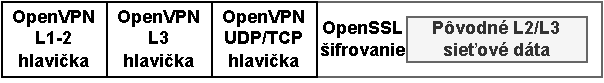
\includegraphics[width=0.9\textwidth]{figures/ovpnptstrc}
	\caption{Zloženie sieťových dát po spracovaní OpenVPN}
	\label{ovpnptstrc}
\end{figure}

Aktuálne používa na šifrovanie AES s 256-bitovou veľkosťou kľúča. V súčasnosti sa OpenVPN považuje za najbezpečnejšiu implementáciu VPN dostupnú pre viacero platforiem. Používateľ ma možnosti vo voľbe protokolu TCP alebo UDP. Podporuje aj prácu s IPv6. OpenVPN nie je kompatabilná s ostatnými protokolmi. Je preto potrebné mať implementáciu na serveri aj klientovi. Nevýhodou je pomerne veľké, energeticky a výpočtovo náročná implementácia.

Viac informácií o tomto komplexnom programe je možné nájsť v \cite{vpntech}, \cite{ovpn} a~priamo na stránke OpenVPN\footnote{https://openvpn.net/faq/what-is-openvpn/}. Z uvedených zdrojov boli aj informácie čerpané. Zdrojový kód je dostupný napríklad na Githube\footnote{https://github.com/OpenVPN/openvpn/}. 
\subsubsection{WireGuard}
WireGuard \cite{wireguardpdf} je najnovší protokol z vyššie uvedených. Pracuje iba na vrstve L3. Jedná sa o implementáciu s voľne dostupným zdrojovým kódom. Vznikol v~roku 2015. Cieľom projektu bolo vytvoriť jednoduchý protokol, ktorý sa ľahko používa, dosahuje vysoké prenosové rýchlosti a poskytuje kvalitnú bezpečnosť pre používateľa. Od roku 2020 sa stal súčasťou Linuxového jadra, konkrétne verzie Linux 5.6 kernel. Aktuálne podporuje veľké množstvo OS vrátane Androidu \cite{android}, Windowsu, MacOS \cite{mac}, OS založené na BSD \cite{bsd} a ďalšie. Za úspešnú implementáciu vďačí WireGuard implemetovaniu svojich funkcionalít do samotných jadier OS, čo značne zrýchľuje spracovanie dát. Samozrejmostou, ostáva aj využitie moderných, extrémne rýchlych kryptografických algoritmov a podpora pre~IPv4 a IPv6. 

Protokoly použité vo WireGuarde sú:
\begin{itemize}
	\item{\textbf{X25519}} \cite{x25519} -- zabezpečuje výmenu kľúčov vďaka kryptografii s eliptickým krivkami \cite{ecc} (ďalej \acrshort{ecc}), ponúka 128-bitovú bezpečnosť s veľkosťou kľúča 256-bitov. Považuje sa za jednu z najrýchlejších kriviek v \acrshort{ecc}.
	\item{\textbf{ChaCha20}} \cite{chacha} -- zabezpečuje symetrické šífrovanie.
	\item{\textbf{Poly1305}} \cite{poly} -- vytvára autentifikačný kód správy (z ang. \textit{Message Authentication codes}). Veľmi častá je kombinácia ChaCha20-Poly1305 za účelom autentizovaného šifrovania s pridruženými dátami (z ang. \textit{Authenticated encryption with associated data}).
	\item{\textbf{SipHash}} \cite{siphash} -- Wireguard používa algoritmus na vytvorenie MAC a jeho následné mapovanie ku kľúčom v hashovacej tabuľke. Hashovacie tabuľky sú známy pojem v~oblasti dátových štruktúr. Ich hlavnou výhodou je vysoká rýchlosť v~porovnaní s~ostatnými možnosťami.  
	\item{\textbf{BLAKE2s}} \cite{blake} -- hashovacia funkcia, rýchlejšia než aktuálne štandardy z~rodiny SHA. 
	\item{\textbf{UDP}} --  protokol na prenos zapuzdrených dát.
\end{itemize} 
WireGuard podporuje aj použitie vopred zdieľaného kľúča za účelom symetrického šifrovania. Dôvodom je pokrok v oblasti kvantových počítačov, ktoré predstavujú riziko pre algoritmy založené na asymetrickom šifrovaní.

Viac informácií o tomto protokole je k dispozícií na \cite{wireguard} a \cite{wireguardpdf}, odkiaľ boli informácie aj čerpané. Zdrojový kód je rozdelený do viacerých repozitárov. Zoznam je dostupný na stránkach Wireguardu\footnote{https://www.wireguard.com/repositories/}.
\section{Zhrnutie VPN sietí}
V~súčasnosti sa využíva VPN aj na súkromné účely. Dôvodov môže byť viacero. Napríklad prístup k lokálne blokovaným doménam, anonymita v internetovom prostredí, zabezpečenie pripojenia a iné. V tomto prípade vstupujú do~popredia tzv. VPN poskytovatelia (z ang. \textit{VPN Providers}), ktorý za poplatok poskytujú výhody pripojenia cez VPN k verejnej sieti. Existujú však aj bezplatné implementácie VPN. Napríklad VPNHood s voľne dostupným zdrojovým kódom\footnote{dostupné na \url{https://github.com/vpnhood/VpnHood}}. 

Na~obrázku \ref{vpnklas2} je schéma zaradenie charakterizovaných protokolov do klasifikácie VPN. Do schémy sme zakomponovali aj DSVPN, ktorá bude predmetom analýzy v ďalších častiach práce.

\begin{figure} [!h]
	\centering
	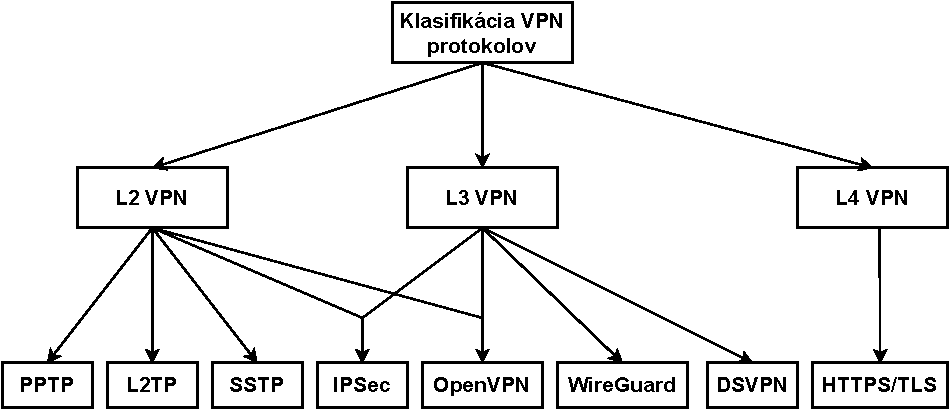
\includegraphics[width=\textwidth]{figures/vpnklas2}
	\caption{Klasifikácia spomenutých VPN protokolov}
	\label{vpnklas2}
\end{figure}

\chapter{Ľahká kryptografia}\label{krypto}
V počítačovej sfére sa čoraz častejšie stretávame so zariadenia, ktorých hardvérové prostriedky a ponúkaný výpočtový výkon sú podstatne nižšie ako v prípade bežne dostupných zariadení na domáce, resp. komerčné použitie. Príkladom môžu byť \acrshort{iot} (z ang. \textit{Internet Of Things}) zariadenia , senzorové uzly, a podobné. Dôležitou vlastnosťou je aj komunikácia medzi sebou alebo inými zariadeniami. V dôsledku toho je nutné riešiť aj otázku zabezpečenia, resp. bezpečnosti takého prenosu dát. 

Kryptografia je oblasť počítačovej vedy, ktorá sa zaoberá práve spomenutou problematikou. Hlavným cieľom je utajiť správu pri jej prenose z bodu A do B. Teda od odosielateľa (tvorcu) správy, až k jej prijímateľovi. Dôsledkom tohto úkonu dochádza k zabezpečeniu 3 hlavných úloh kryptografie:
\begin{itemize}
	\item \textbf{ochrana osobných údajov} (dôvernosť) -- z ang. \textit{Data Privacy}, 
	\item \textbf{autenticita údajov} (prišla z miesta, ktoré sa uvádza ako zdroj dát)  -- z ang. \textit{Data Authenticity},
	\item \textbf{integrita údajov} (nebolia upravená počas prenosu)  -- z ang. \textit{Data Integrity}.
\end{itemize} 
Pojem kryptografia vznikol už pomerne dávno a bol už viackrát charakterizovaný. Z toho dôvodu sa tejto problematike ďalej nebudeme venovať. Viac informácií je možné nájsť v \cite{levicky}. 

V súčasnosti má používateľ možnosť vybrať si zo širokej ponuky kryptografických algoritmov. Výber je volený na základe potrebnej funkcionality, ktorú sa snažíme implementovať. Napríklad za účelom symetrického šifrovania by sme mohli použiť \acrshort{aes} \cite{aes} (z ang. \textit{Advanced Encryption Standard}), ktorý je aktuálne používaný ako štandardný kryptografický algoritmus. Detailný opis jednotlivých blokov a postupov použitých v AES-e, je obsahom rôznych publikácií. Viac informácií o problematike nájde čitateľ napríklad v \cite{levicky}.

V prípade zariadení spomenutých v úvode kapitoly, však môže nastať problém s výpočtovým výkonom pri realizácií algoritmov. Vo výsledku trvá vykonávanie funkcionality omnoho dlhšie a je aj energeticky náročnejšie ako v prípade normálnych zariadení. V roku 2005 bol prvýkrát definovaný pojem, z ang. \textit{Lightweight Cryptography}. Konkrétne v práci \cite{lwc}. Vrámci tejto práce voľne preložíme tento pojem ako \textbf{Ľahká kryptografia} (ďalej \acrshort{lwc}). 

\acrshort{lwc} algoritmy sú mnoho násobne efektívnejšie ako súčasne používané konvenčné kryptografické štandardy. Dôvodom je ich vysoká efektívnosť a nízky počet potrebných procesorových inštrukcií na vykonanie cielenej funkcionality. V súčasnosti je častým javom použitie označenia \textit{lightweight} pre ľubovoľný kryptografický algoritmus. Jedná sa o implementácie, ktoré svojimi vlastnosťami spĺňajú základné požiadavky LWC. Tie boli definované samotnými autormi už v diele \cite{lwc}. Sú nimi: 
\begin{itemize}
	\item{\textbf{minimalizácia spotreby zdrojov zariadenia}} -- veľkosť kódu, používaných dát a spotreby energie,
	\item{\textbf{poskytnutie dostatočné vysokého stupňa bezpečnosti}},
	\item{\textbf{odolnosť voči útoku cez postranné kanály} -- z ang. \textit{side-channel attack}}, napríklad útokom na analýzu výkonu a na časovanie, 
	\item{\textbf{jednoduchá implementácia a efektívnosť,}}
	\item{\textbf{nízke pamäťové nároky}} -- z ang. \textit{low memory footprint}.
\end{itemize}

V práci budeme tieto algoritmy označovať ako \textit{Lightweight Cryptographic Algorithm} (ďalej \acrshort{lwca}).
\acrshort{lwca} tvoria kryptografické algoritmy, ktoré splňajú vyššie stanovené vlastnosti a teda je možné ich aj nasadiť do tzv. \textit{low resource} zariadení. V~závislosti od výslednej implementácie sa sledujú požiadavky na daný algoritmus. V prípade hardvérovej implementácie najväčšiu úlohu pri tvorbe optimálneho algoritmu zohráva energetická spotreba a potrebná veľkosť čipu. Na druhej strane, pri softvérovej implementácií je dôležitým aspektom veľkosť algoritmu a jeho využitie RAM pamäte. Čím sú uvedené parametre nižšie, tým výhodnejší je nasadenie daného algoritmu pre cieľové zariadenie. V prípade výpočtovo obmedzených zariadení sa pri výslednej implementácií \acrshort{lwca} môžeme stretnúť aj s kompromisom medzi ponúknutou bezpečnosťou a efektivitou.

V rámci tejto kapitoly si predstavíme jeden z novších \acrshort{lwca} algoritmov. Konkrétne balík Xoodyak s kryptografickou permutáciou XOODOO \cite{tkecak} a jeho použitie. Xoodyak sa stal jedným z 10 finalistov v \acrshort{lwc} štandardizačnom procese Národného inštitútu pre štandardy a technológie (ďalej \acrshort{nist}) \cite{lwc3}. Vo februári roku 2023 bol za víťaza zvolený algoritmus Ascon \cite{ascon}.

Viac podrobností nájde čitateľ v \cite{lwc}, \cite{lwc2} a \cite{lwc3}, odkiaľ boli aj informácie z~tejto kapitoly čerpané. 
        
\section{Kryptografická permutácia XOODOO a jej variácie}
Permutácia je operácia, ktorá mení pozíciu vstupných prvkov, tak aby vo výsledku vzniklo nová usporiadaná množina. Kryptografické permutácie sú špeciálne navrhnuté matematické algoritmy, tak aby bolo možné využiť ich za účelom šifrovania a dešifrovania. Operácie vykonané v takýchto permutáciách musia byť invertibilné. Kryptografické permutácie tvoria základný stavebný blok pri následnej tvorbe ďalších kryptografických blokov. Množina základných stavebných blokov sa v kryptografii spoločne označuje ako kryptografické primitíva (ďalej \acrshort{kp}). Príkladom môžu byť hašovacie funkcie, generátory náhodných čísel a podobne. Viac informácií nájde čitateľ v \cite{kp}.  
 
XOODOO je sada 384-bitových kryptografických permutácií parametrizovaných počtom kôl. Funkcia kola/rundy (z ang. \textit{round}) funguje na 12 slovách (z ang. \textit{words}) po 32 bitoch. Vďaka tomu je efektívna aj na menej výkonných procesoroch nižšej triedy. Vytvoril ju tím Keccak \cite{kecak}, ktorý stojí za viacerými úspešnými kryptografickými algoritmami. Napríklad hashovacie funkcie z rodiny SHA-3 a iné -- \cite{kecsup}. XOODOO algoritmus vznikol po vytvorení tzv. Kravatte autentizačno-šifrovacieho algoritmu \cite{kravatte}, založené na Keccak-p permutácií \cite{keccakp}. Ten sa ukázal ako dostatočne rýchly na širokom spektre platforiem. Avšak nezapadá do kategórie \acrshort{lwca}.

Tím Keccak vypracoval nové riešenie založené na ich Keccak-p dizajne a permutačnom algoritme Gimli \cite{bernstein2017gimli}. Vo výsledku autori zlúčili lepšie realizované prvky z oboch algoritmov do jedného celku. Primárny problém samotnej permutácie Gimli bol v slabom prejave zmeny výstupu po malých zmenách vo vstupnej správe. Táto vlastnosť sa v kryptografii označuje pomocou anglického pojmu, tzv. \textit{propagation properties}\footnote{Cieľom je aby aj zmena jedného bitu na vstupe, ovplyvnila čo najviac bitov vo výstupe -- tzv. \textit{Lavínový efekt}}. Novo-vzniknuté riešenie autori pomenovali XOODOO. Na základe rôznych variácií tohto kryptografického primitíva sa im následne podarilo vytvoriť sadu vysoko efektívnych kryptografických funkcií. 
Medzi sady, ktorých jadro tvorí XOODOO, patrí Xoodyak a Xoofff. Xoofff pozostáva zo zlúčenia Farfalle konštrukcie \cite{farfalle} so XOODOO permutáciou. 

Xoodyak má, na rozdiel od Xoofff, duplexovú konštrukciu \cite{duplex}. Vo výsledku máme ľahko prenosnú, všestrannú, kryptografickú knižnicu. Je vhodná do výkonovo obmedzených prostredí. Môže sa použiť pre väčšinu kryptografických funkcií, ktoré používajú symetrický kľúč. Napríklad hashovanie, šifrovanie, výpočet MAC alebo autentizované šifrovanie. O kvalite riešenia napovedá aj fakt, že sada Xoodyak je jedným z 10 finalistov v oblasti ľahkej kryptografie NIST štandardizačného procesu, ktorý pozostával z 3 predchádzajúcich kôl. Ich úlohou bolo vybrať najlepšie algoritmy zo všetkých prihlásených.

V rámci tejto kapitoly opíšeme kryptografické primitívum XOODOO a následne balík Xoodyak. Informácie o téme boli čerpané z týchto zdrojov: \cite{tkecak}, \cite{xd}, \cite{xcb}, \cite{xoodoocb}, \cite{xdupdate},\cite{xdr1}.
\subsection{XOODOO permutácia}
XOODOO je permutácia, definovaná počtom rúnd. Má klasickú iteračnú štruktúru. Teda opakovane sa vola rundová funkcia s aktuálnym stavom. Pre pochopenie operácií je nutné pochopiť určité označenie použité v algoritme.

Stav -- \textbf{state}, pozostáva z 3 rovnako veľkých horizontálnych rovín -- \textbf{planes}\footnote{v jednej rovine je 128 bitov}. Každá z týchto rovín obsahuje štyri paralelne 32-bitové pruhy -- \textbf{lanes})\footnote{v jednom pruhu je 32 bitov}. Okrem tejto charakteristiky je možné opísať stav ako množinu zloženú zo stĺpcov -- \textbf{columns}\footnote{v jednom stĺpci je 12 bitov}, pričom jeden stĺpec obsahuje 4 bity v jednej rovine. Stav je teda tvorený zo stĺpcov usporiadaných v poli o rozmere $4\times3\times32 = 384$ bitov. Posledná položka na opis stavu sú tzv. listy -- \textbf{sheets}\footnote{v jednom liste je 96 bitov}. List sa skladá z 3 na sebe uložených pruhov. Uvedené pojmy sú znázornené pomocou obrázka \ref{xoodooterm}, ktorý bol prevzatý z \cite{xcb}.

\begin{figure}[!h]
	\centering
	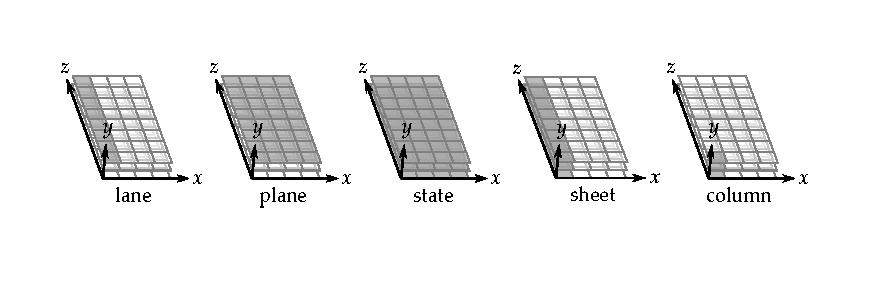
\includegraphics[width=1\textwidth]{figures/xoodooTerminology}
	\caption{Grafické znázornenie terminológie využitej v kryptografickej permutácii XOODOO \cite{xcb}}
	\label{xoodooterm}
\end{figure}

Roviny majú index $y$. Index $y=0$ zodpovedá spodnej rovine a vrchná rovina má index $y=2$. Bit je označený s indexom $z$ vrámci množiny pruhov. List označujeme pomocou indexu $x$. Pozícia pruhu v stave je definovaná pomocou dvoch súradníc $(x,y)$. Konkrétny bit je možné reprezentovať v stave pomocou trojice súradníc $(x,y,z)$. Pri určení stĺpca sú potrebné 2 súradnice $(x,z)$. Pred spustením samotného algoritmu musí používateľ vykonať mapovanie 384-bitovej správy voči horizontálnym rovinám. Tento úkon sa realizuje pomocou vzorca \ref{index}.

\begin{equation}\label{index}
	i=z+32(x+4y)
\end{equation}
Výhodou XOODOO je, že celý stav, 384 bitov, dokáže byť uložený v 12 registroch po 32 bitov. Vďaka tomu ideálne vyhovuje nízko výkonným 32-bitovým zariadeniam.

Rundová funkcia pozostáva z 5 krokov:
\begin{enumerate}
	\item miešanie vrstvy -- z ang. \textit{a mixing layer $\theta$}, 
	\item posun rovín -- z ang. \textit{a plane shifting $\rho_{west}$}, 
	\item pridanie rundových konštánt -- z ang. \textit{the addition of round constants $\iota$},
	\item nelineárna vrstva -- z ang. \textit{a non-linear layer $\chi$},
	\item posun rovín -- z ang. \textit{an another plane shifting $\rho_{east}$}.
\end{enumerate}
Opis jednotlivých krokov je znázornený pomocou obrázkov \ref{xoodoochi}, \ref{xoodooml}, \ref{xoodooshift} ktoré sú prevzatý z \cite{xcb}.  

% TODO: \usepackage{graphicx} required
\begin{figure}[h!]
	\centering
	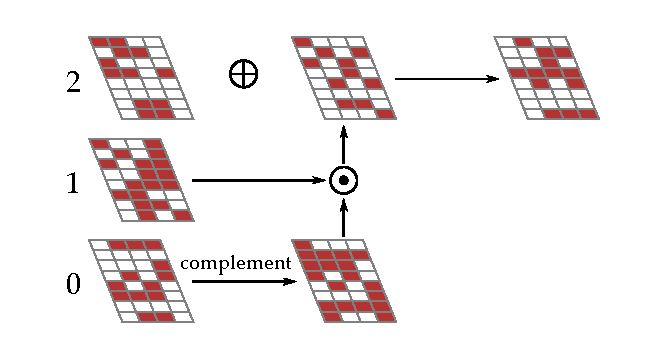
\includegraphics[width=0.6\textwidth]{figures/xoodoochi}
	\caption{Grafické znázornenie operácie $\chi$ \cite{xcb}}
	\label{xoodoochi}
\end{figure}
% TODO: \usepackage{graphicx} required
\begin{figure}[h!]
	\centering
	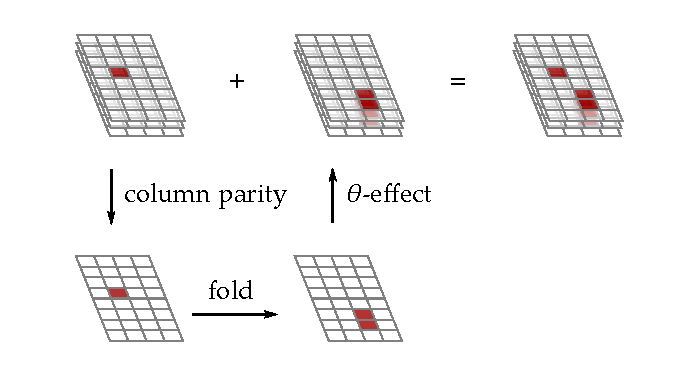
\includegraphics[width=0.6\textwidth]{figures/xoodooml}
	\caption{Grafické znázornenie operácie $\rho$ \cite{xcb}}
	\label{xoodooml}
\end{figure}
% TODO: \usepackage{graphicx} required
\begin{figure}[h!]
	\centering
	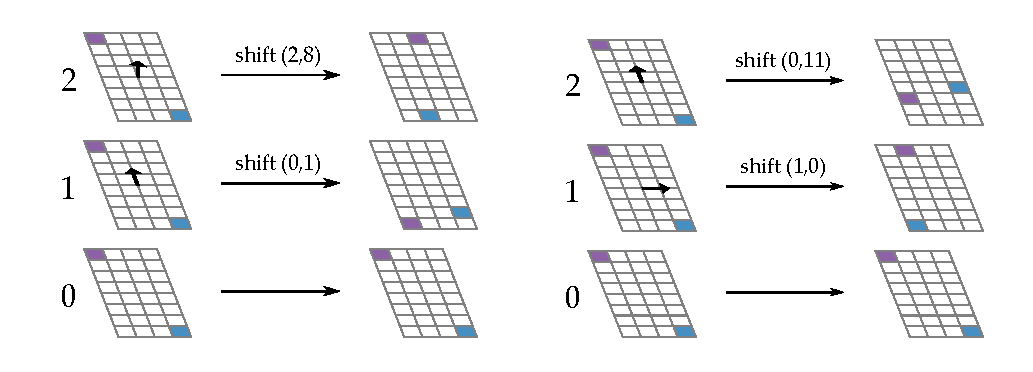
\includegraphics[width=0.9\linewidth]{figures/xoodooshift}
	\caption{Ilustrácia miešania vrstiev $\rho_{west}$ (vľavo) a $\rho_{east}$ (vpravo)\cite{xcb}}
	\label{xoodooshift}
\end{figure}
V~obrázku \ref{xoodooshift} je posun realizovaný na každom bite. V~obrázku sú ilustrované len posuny 2 bitov. 
   
Tabuľka \ref{tab1} vysvetľuje jednotlivé operácie, ktoré sa v algoritme používajú. Algoritmus permutácie je následne znázornený pomocoou obrázku \ref{xoodooalgo}. Súčasťou implementácie sú aj tak zvané rundové konštanty. Tie je možné vidieť v tabuľke \ref{tab2}. Uvedené ilustrácie boli prevzaté z dokumentu \cite{xcb}.

\begin{figure}[!h]
	\centering
	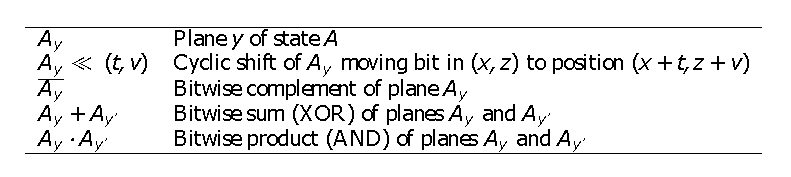
\includegraphics[width=1.0\textwidth]{figures/tab1}
	\caption{Charakteristika operácií v algoritmickom zápise kryptografickej permutácie XOODOO \cite{xcb}}
	\label{tab1}
\end{figure}

\begin{figure}[h!]
  	\centering
  	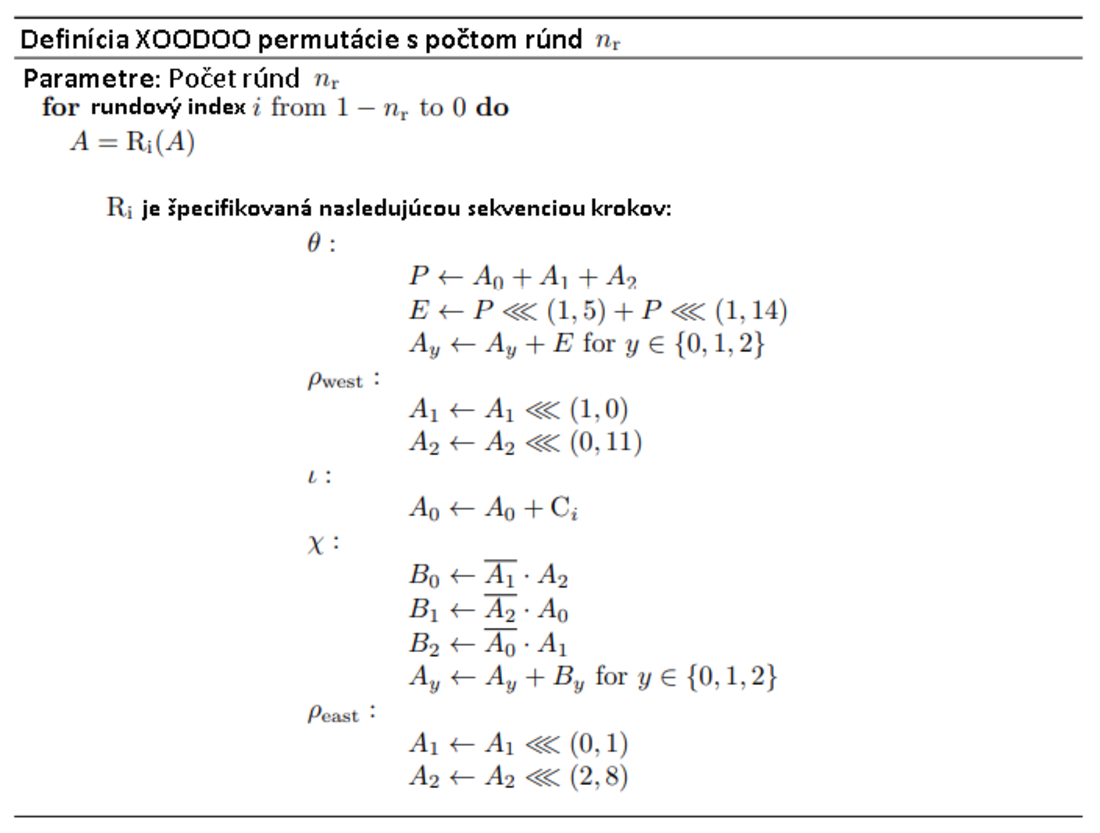
\includegraphics[width=1.0\textwidth]{figures/xoodooalgo}
  	\caption{Algoritmický zápis kryptografickej permutácie XOODOO \cite{xcb}}
  	\label{xoodooalgo}
\end{figure}


\begin{table}[!h]
	\centering
	\resizebox{0.25\textwidth}{!}{%
		\begin{tabular}{c|c} 
			\multirow{1}{*}{\bfseries$i$}&
			\multicolumn{1}{c}{ \bfseries$c_i$}   
			\\\hline\hline
			 0 
			&  0x00000012
			\\
			 -1
			&  0x000001A0
			\\
			 -2 
			&  0x000000F0
			\\
			 -3 
			&  0x00000380
			\\
			 -4 
			&  0x0000002C
			\\
			 -5 
			&  0x00000060 
			\\
			 -6 
			& 0x00000014
			\\
			 -7 
			& 0x00000120
			\\
			 -8 
			&  0x000000D0
			\\
			 -9 
			&  0x000003C0
			\\
			 -10
			&  0x00000038
			\\
			 -11 
			&  0x00000058
			\\	
		\end{tabular}
	}
	\caption{Súbor rundových konštánt kryptografického algoritmu \\ XOODOO \cite{xcb}}\label{tab2}
\end{table}


\subsection{Kryptograficý balíček Xoodyak} 
Xoodyak možno považovať za všestranný kryptografický nástroj. Je vhodný pre väčšinu operácií využívajúcich symetrický kľúč. Napríklad generovanie pseudonáhodných bitov, autentizáciu, šifrovanie a iné. Tím Keccak použil pri návrhu duplexnú konštrukciu. Konkrétne variant s plným stavom a využitím kľúča. Tento dizajn označujeme ako \acrfull{fskd}. Viac o tejto konštrukcii si čitateľ môže prečítať v \cite{duplex}.
Operačný režim, v ktorom Xoodyak pracuje sa nazýva Cyklista -- z ang. \textit{Cyclist}. Tento názov získal ako opozitum k pomenovaniu režimu Motorista (z ang. \textit{Motorist}), ktorý je možné nájsť v Keyak schéme \cite{keyak}. Narozdiel od uvedeného balíka Keyak, nie je Xoodyak limitovaný len na autentizované šifrovanie. Je jednoduchší hlavne kvôli tomu že neobsahuje paralelné varianty.

\subsubsection{Režim Cyklista}\label{cyklista}
Režim Cyklista funguje na princípe kryptografických permutácií $f$, teda zmeny usporiadania bitov za pomoci tajného kľúča a matematických operácií. Parametrami sú veľkosti blokov $R_{hash}$, $R_{kin}$, $R_{kout}$ a veľkosť račety, resp. západky (z ang. \textit{the ratchet size}) \cite{ratchet} $\ell_{ratchet}$. Uvedený pojem sa v kryptografii používa vo forme obrazného pomenovania. Cieľom je poukázať na jednoduchý pohyb vpred, ale s ťažkým, resp. zložitejším pohybom naspäť. Dôležité je, že uvedený scenár je vyvolaný zámerným dizajnom. Šírka permutácie $b'$ je definovaná pomocou vzorca (\ref{index2}). Všetky uvedené parametre sú v bajtoch. Pre označenie prázdneho slova budeme používať $E$.
\begin{equation}\label{index2}
	max(R_{hash}, R_{kin}, R_{kout}) + 2 \leq b'
\end{equation} 

Cyklista operuje v dvoch režimoch -- \textbf{hašovací a kľúčový} (z ang. \textit{hash and keyed mode}). 
Inicializácia prebieha pomocou príkazu \lstinline|CYCLIST(K,id,counter)|. Ak sa parameter $K$ rovná prázdnemu slovu $E$, tak potom nastane spustenie v hašovacom režime. Aktuálne nie je do implementácie zakomponovaná možnosť zmeny režimu po inicializácií. Vývojári však túto vlastnosť nevylúčili pre prípadné aktualizácie balíka.  


Dostupné funkcie závisia od režimu, v ktorom sa  Cyklista spúšťa. Medzi ne~patria \lstinline|ABSORB()| a \lstinline|SQUEEZE()|. Možno ich volať v oboch režimoch, zatiaľ čo funkcie \lstinline|ENCRYPT()|, \lstinline|DECRYPT()|, \lstinline|SQUEEZEKEY()| a \lstinline|RATCHET()| sú dostupné len pre kľúčový režim. Účel každej funkcie je nasledujúci:
\begin{itemize}
	\item \lstinline|ABSORB(X)| absorbuje vstupný reťazec X,
	\item $C$ $\gets$ \lstinline|ENCRYPT(P)| zašifruje P do C a absorbuje P,
	\item $P$ $\gets$ \lstinline|DECRYPT(C)| dešifruje C do P a absorbuje P,
	\item $Y$ $\gets$	\lstinline|SQUEEZE(L)|  vytvára L-bajtový výstup, ktorý závisí od doteraz absorbovaných dát,
	\item $Y$ $\gets$	\lstinline|SQUEEZEKEY(L)| funguje ako \lstinline|SQUEEZE(L)|, ale používa sa za účelom generovania odvodeného kľúča,
	\item \lstinline|RATCHET()| transformuje stav na nevratný tak, aby sa zabezpečila dopredná bezpečnosť (z ang. \textit{Forward secrecy}) \cite{fsec}. 
\end{itemize}

Stav bude závisieť od postupnosti volaní funkcií a od jeho vstupných reťazcov. Presnejšie povedané, zámerom je, že akýkoľvek výstup závisí od postupnosti všetkých vstupných reťazcov a volaní, tak že akékoľvek dva nasledujúce výstupné reťazce budú výstupom rôznych domén. Napríklad volanie \lstinline|ABSORB(X)| znamená, že výstup bude závisieť od reťazca $X$. Na druhej strane \lstinline|ABSORB()| vo funkcii \lstinline|ENCRYPT(P)| vytvorí výstup závislý aj od $P$ z funkcie šifrovania. Okrem uvedených závislostí ovplyvňujú výstup aj iné dizajnové riešenia. Príkladom je minimalizácia pamäťových požiadaviek. Vo výsledku teda výstup závisí od počtu predchádzajúcich volaní funkcie \lstinline|SQUEEZE()| a predtým spracovaných textov pomocou funkcií \lstinline|ENCRYPT()| a \lstinline|DECRYPT()|. Viac informácií o režime je dostupných v kapitole 7.2, publikácie \cite{xcb}.
Algoritmický zápis jednotlivých funkcií a doplňujúce informácie o režime Cyklista je možné nájsť v \cite{xdr2}, konkrétne v kapitole 2.2. 

\subsubsection{Definícia a bezpečnosť}
Xoodyak je definovaný pomocou operatívneho režimu Cyklista nasledovne:
\begin{equation}
	CYCLIST[f,R_{hash},R_{kin},R_{kout},L_{ratchet}]
\end{equation} 
Kde jednotlivé parametre majú veľkosti:
\begin{enumerate}
	\item $f$ -- permutácia XOODOO so šírkou 48 bajtov (384 bitov),
	\item $R_{hash}$ -- 16 bajtov,
	\item $R_{kin}$ -- 44 bajtov,
	\item $R_{kout}$ -- 24 bajtov,
	\item $L_{ratchet}$ -- 16 bajtov.  
\end{enumerate}
Takto definované parametre algoritmu dokážu poskytnúť 128-bitovú bezpečnosť v oboch režimoch Cyklistu. Samozrejmosťou je, že v prípade kľúčového režimu, musí byť veľkosť kľúča rovná alebo väčšia ako 128 bitov. Viac informácií o kryptografickej bezpečnosti algoritmov je možné nájsť v \cite{sec}.

Viac informácií o bezpečnosti Xoodyak-a je možné nájsť v \cite{xcb} (kapitola 7.3) a \cite{xdr2}, odkiaľ boli informácie čerpané.

\subsection{Možnosti použitia Xoodyak algoritmu}
Obsahom tejto podkapitoly sú uvedené postupy ako a za akých okolností je daný balík možné použiť. 
\subsubsection{Použitie hašovacieho režimu}
Xoodyak sa dá aplikovať ako hašovacia funkcia. Konkrétne je možné ju použiť ako funkciu na rozšírenie výstupu (z ang. \textit{eXtendable-Output Function}) (ďalej \acrshort{xof}). Nominálne, resp. nie bežné použitie by v tomto prípade bolo nasledujúce: 
\begin{lstlisting}[language=bash,mathescape=true]
	CYCLIST($E$,$E$,$E$) //spustenie v hašovacom režime,
 	ABSORB($X$)        //absorpcia vstupného reťazca X,
 	SQUEEZE($L$)       //vytvára L-bajtový výstup, 
	     	          //závislý od doteraz absorbovaných dát.
\end{lstlisting}
V tomto prípade by sa kryptografická bezpečnosť algoritmu pohybovala v závislosti od veľkosti výstupu L. Konkrétne v intervaloch:
\begin{itemize}
	\item{\textbf{odolnosť voči kolízií}} -- z ang. \textit{collision resistance} \cite{cr}, min(8L/2, 128) bitov,
	\item{\textbf{odolnosť voči }} -- z ang. \textit{preimage and second preimage resistance} \cite{pa}, min(8L, 128) bitov,
	\item{\textbf{odolnosť voči}} -- z ang. \textit{m-target preimage resistance} \cite{pa}, min(8L - log m, 128) bitov.
\end{itemize}
Bežná je však absorpcia sekvencie viacerých reťazcov.

\subsubsection{Použitie kľúčového režimu}
Inicializácia režimu začína použitím príkazu \lstinline|CYCLIST(K,id,counter)|. Autori uviedli celkovo 6 spôsobov použitia. V nich sa opisuje význam parametrov $id$, $counter$ $nounce$ a podobne aj možnosti použitia funkcií, spomenutých na začiatku podkapitole.
\begin{itemize}
	\item{\textbf{Použitie na zabránenie viac-cieľového útoku}} -- z ang. \textit{Two ways to counteract multi-target attacks},
	\item{\textbf{Tri spôsoby spracovania jednorázového kľúča}} -- z ang. \textit{Three ways to handle the nonce},
	\item{\textbf{Autentizované šifrovanie}} -- z ang. \textit{Authenticated encryption},
	\item{\textbf{Autentizované relačné šifrovanie}} -- z ang. \textit{Session authenticated encryption},
	\item{\textbf{Použitie funkcie \lstinline|RATCHET()|}} -- z ang. \textit{Ratchet},
	\item{\textbf{Pohyblivé subkľúče}} -- z ang. \textit{Rolling subkeys}.
\end{itemize}

\textbf{Použitie na zabránenie viac-cieľového útoku} -- $id$ parameter je voliteľný identifikátor kľúča $K$. Pre každý tajný kľúč by mal byť jedinečný. Ponúka možnosť zabránenia viac-cieľovým útokom. Jedná sa o útok na viacero používateľov daného kryptografického systému, resp. viacero kľúčov používateľa. Viac o tomto útoku je možné nájsť v \cite{mta}. V prípade použitia $id$ parametra algoritmus rozšíri veľkosť kľúča. Následne pri vyhľadávaní kľúčov nedochádza k degradácií bezpečnosti a~veľkosť tajného kľúča môže ostať 128 bitov. Týmto spôsobom bude zachovaná aj rovnaká bezpečnosť systému pred útokom. 
Príklad za účelom šifrovania správy $P$ za pomoci tajného kľúča $K$ s $id$, je na nasledujúci:
\begin{lstlisting}[language=bash, mathescape=true]
	CYCLIST($K$,$id$,$E$)
	ABSORB(nounce)
	$C$ $\gets$ ENCRYPT($P$).
\end{lstlisting}
\textbf{Tri spôsoby spracovania jednorázového kľúča} -- 3. parameter pri inicializácií režimu cyklista je \textit{counter}, resp. počítadlo. Jedná sa o dátový prvok vo forme bajtového reťazca, ktorý môže byť inkrementovaný. Spracúva sa po jednej číslici. Vďaka tomu sa obmedzuje počet informácií, ktoré vie útočník využiť pre rôzne vstupy. Pri inicializácií používateľ zvolí veľkosť počítadla v intervale $2 \leq B \leq 256$. Predpokladá sa, že počítadlo je reťazec z množiny $\mathbb{Z^*_B}$. Potom ak je počítadlo inicializované ako prázdny reťazec, tak množina všetkých možných hodnôt po inkrementácií je $\mathbb{Z^1_B}$. Pri každom ďalšom navýšení sa zvýši hodnota za $*$. Spracovanie prebieha od najvýznamnejšieho bitu. Čím menšia je hodnota $B$, tým menší je počet možných vstupov pri každej iterácií permutácie. Vďaka tomu je zabezpečená lepšia ochrana pred tzv. z ang \textit{Power analysis} \cite{paa} útokmi a jeho variantami. Za~účelom zamedzenia týchto útokov sa používa \lstinline|ABSORB(nounce)| v prípade ak si počítadlo pri inicializácií zvolíme prázdny reťazec $E$. 

\textbf{Autentizované šifrovanie} -- za účelom autentizovaného šifrovanie je Xoodyak možné použiť nasledovne:
\begin{lstlisting}[language=bash,mathescape=true]
	CYCLIST($K$,nonce,$E$)
	ABSORB($A$)
	$C$ $\gets$ ENCRYPT($P$)
	$T$ $\gets$ SQUEEZE($t$)
	return ($C$,$T$)
\end{lstlisting}
Pričom $K$ je tajný kľúč s pridruženým jednorázovým heslo a dátami $A$ k heslu. Z~týchto údajov sa získa autentizačný tag $t$. Jeho veľkosť je rovná 16-bajtom. V~prípade dešifrovania by postupnosť volaní vyzerala nasledovne: \\  
\begin{lstlisting}[language=bash,mathescape=true]
	CYCLIST($K$,nonce,$E$)
	ABSORB($A$)
	$C$ $\gets$ ENCRYPT($P$)
	$T$ $\gets$ SQUEEZE($t$)
	if $T = T'$ then 
		return $P$, 
	else 
		return $\bot$ 	//vyjadrenia hodnoty false 
\end{lstlisting}
Kryptografická bezpečnosť takto implementovaného šifrovania je minimom z uvedených hodnôt $min(184,K,8t)$.

\textbf{Autentizované relačné šifrovanie} -- pracuje so sekvenciou správ a autentizačných tagov. V princípe sa opakuje viacero blokov z predchádzajúcej možnosti použitia. Prvé volanie je rovnaké ako v predchádzajúcom príklade. Implementácia však zahŕňa aj možnosť vytvoriť tag bez toho aby bolo nutné použiť funkcie
\lstinline|ABSORB()|, \lstinline|ENCRYPT()| alebo obe súčasne pred volaním \lstinline|SQUEEZE()|. Aj napriek tomu bude možné vytvoriť nový tag na základe predchádzajúcich dát, uložených v pamäti. 	

\textbf{Použitie funkcie \lstinline|RATCHET()|} -- používateľ môže v režime kľúča kedykoľvek volať funkciu \lstinline|RATCHET()|. Volanie spôsobí prepísanie časti stavu s nulami. Vďaka tomu je nemožné vypočítať stav pred volaním funkcie \lstinline|RATCHET()|. Týmto spôsobom je možné zťažiť snahu pri pokuse obnoviť vnútorný stav, napríklad pri útoku postrannými kanálmi. \lstinline|RATCHET()| je možné použiť obdobne aj pri autentizovanom šifrovaní. Konkrétne pred alebo za funkciou vytvárania tagu \lstinline|SQUEEZE()|. 
\begin{lstlisting}[language=bash,mathescape=true]
	CYCLIST($K$,nonce,$E$)
	ABSORB($A$)
	$C$ $\gets$ ENCRYPT($P$)
	RATCHET()	  //príklad volania pred
	$T$ $\gets$ SQUEEZE($t$)
	RATCHET()   //príklad volania za
\end{lstlisting} 
Obidva spôsoby majú svoje výhody. Volanie pred vytváraním tagu je najfektívnejšie. Dôvodom je, že vďaka tomu je potrebné len jedno extra volanie permutácie. V prípad volania funkcie \lstinline|RATCHET()| za \lstinline|SQUEEZE()| sa šifrovaný text prenáša, funkcionalita \lstinline|RATCHET()| je vykonaná asynchrónne a algoritmus môže spracovať ďalšiu správu, určenú na šifrovanie. 

\textbf{Pohyblivé subkľúče} -- je alternatíva k použitiu dlhodobého tajného kľúča $K$ s~inkrementovanými pridruženým jednorázovým kľúčom $nounce$ alebo identifikátorom kľúča $id$. Subkľúč/e sa vytvára/jú pomocou funkcie \lstinline|SQUEZEEKEY()|. Pri~šifrovaní je teda možné nahradiť procesy inkrementácie a ukladania jednorázových hesiel pri každom použití  $K$, pomocou použitia pohyblivých subkľučov.

\begin{lstlisting}[language=bash,mathescape=true]
	$K_1 \gets K$ and $i \gets 1 $	   //inicializacia tajneho kluca
	while condition do 
	CYCLIST($K$,$E$,$E$)	//inicializácia novej Xoodyak inštancie
	$K_{i+1} \gets$ SQUEEZEKEY($\ell_{sub}$) 
	RATCHET()	      //volitelne
	ABSORB($A_i$)
	$C_i \gets$ ENCRYPT($P_i$)     //sifrovanie
	$T_i \gets$ SQUEEZE($t$)      //vypocet tagu
	$\implies$ output($C_i$,$T_i$) //caka na dalsiu správu
	$i \gets i + 1$
\end{lstlisting}     
Parameter $\ell_{sub}$ je vo veľkosti 32 bajtov (256 bitov). Táto veľkosť by mala byť dostatočná aby sa zabránilo kolíziám za predpokladu, že v subkľúčoch nevznikla kolízia. Použitie týmto spôsobom ponúka odolnosť voči útokom cez postranné kanály. Tajný kľúč nie je po dodávke prvého subľúča používaný. Vďaka tomu nie je ani vystavený možnému útoku. Každým ďalším šifrovaním sa mení aj použitý kľúč na šifrovanie, čo veľmi sťažuje možnosti ďalšej analýzy. 
 
\subsubsection{Použitie za účelom autentizovaného šifrovania s bežným heslom}
Protokoly na výmenu kľúčov, ako napríklad Diffie-Hellman, poskytujú vo výsledku bežný tajný kľuč. Pred symetrickým šifrovaním je však potrebná jeho úprava. Za týmto účelom je možné použiť Cyklistu v hašovacom režime. Následne po spracovaní bežného kľúča použijeme odvodený kľuč na spustenie režimu kľúča. Funkcionalita je jednotlivých volaní je znázornená nižšie. \newpage
\begin{lstlisting}[language=bash,mathescape=true]
	CYCLIST($E$, $E$, $E$)         //hasovaci rezim
	ABSORB($ID$)              //ID pouziteho protokolu
	ABSORB($K_A$)              //verejny kluc A
	ABSORB($K_B$)              //verejny kluc B 
	ABSORB($K_{AB}$)              //tajny kluc 
	$K_D \gets$ SQUEEZE($\ell$)
	
	CYCLIST($K_D$, $nonce$, $E$)       //rezim kluca
	ABSORB($A$)
	$C \gets$ ENCRYPT($P$)
	$T \gets$ SQUEEZE($t$)
	return ($C$, $T$)
\end{lstlisting} 
Ak platí $\ell \leq R_{hash}$, tak implementácia dokáže efektívne zreťaziť tajný kľúč $K_D$ a reinicializovať cyklistu \lstinline|CYCLIST(|$K_D$,$E$,$E$\lstinline|)|. Dôvodom je, že tajný kľúč je už súčasťou stavu permutácie. Je len potrebné nastaviť zvyšné parametre. 

\subsection{Overenie správnosti implementácie algoritmu pomocou testovacích vektorov}
Povinnosťou tvorcov kryptografických algoritmov pri štandardizačnom procese NIST je dodať referenčnú implementáciu algoritmu, dostupnú na \cite{vektory}. Pomocou nej si vieme overiť správnosť iných implementácií. Nás však zaujala pomerne jednoduchá implementácia, ktorá obsahuje aj overenia správnosti algoritmu. Jedná sa o program s názvom Xoocycle \cite{xootest}, ktorý má voľne dostupný kód napísaný v jazyku C. Implementácia obsahuje XOODOO permutáciu spoločne s funkciami z balíka Xoodyak. Používateľ si teda môže vyskladať použitie aj podľa vyššie opísaných možností použitia. Zároveň obsahuje testovací zdrojový kód \lstinline|xootest.c| na overenie výstupu. Po úprave vstupu a následnej kompilácií je tak možné overiť správnosť výstupu implementácie. Archív s uvedenými zdrojovými kódmi je dostupný v \cite{xootest}. Uvedený archív prikladáme spoločne s referenčnou implementáciou do Prílohy A.1.       